% % % % % % % % % % % % % % % % % % % % % % % % % % % % % % % % % % % % % % % % % % % %
%                                                                                     %
% Short Sectioned Assignment LaTeX Template Version 1.0 (5/5/12)                      %
% This template has been downloaded from: http://www.LaTeXTemplates.com               %
%                                                                                     %
% Original author:  Frits Wenneker (http://www.howtotex.com)                          %
%                                                                                     %
% Modified by: Fco Javier Sueza Rodríguez (fcosueza@disroot.org)                      %
%                                                                                     %
% Changes:                                                                            %
%	    - Custom Chapters, Sections and Subsections (titlesec package)                %
%           - Document type scrbook (oneside)                                         %
%           - Use babel-lang-spanish package and marvosym                             %
%           - Use hyperref, enumitem, tcolorbox and glossaries packages               %
%           - Use Time New Roman (mathptmx), Helvetic and Courier fonts               %
%                                                                                     %
% License: CC BY-NC-SA 3.0 (http://creativecommons.org/licenses/by-nc-sa/3.0/)        %
%                                                                                     %
% % % % % % % % % % % % % % % % % % % % % % % % % % % % % % % % % % % % % % % % % % % %

%-----------------------------------------------%
%	              Packages                  %
%-----------------------------------------------%

\documentclass[paper=a4, fontsize=11pt, oneside]{scrbook}

% ---- Text Input/Output ----- %

\usepackage[T1]{fontenc}
\usepackage[utf8]{inputenc}
\usepackage{mathptmx}
\usepackage[scaled=.92]{helvet}
\usepackage{courier}
\usepackage[indent=12pt]{parskip}

\usepackage{geometry}
\geometry{verbose,tmargin=3cm,bmargin=3cm,lmargin=2.6cm,rmargin=2.6cm}

% ---- Language ----- %

\usepackage[spanish]{babel}
\usepackage{marvosym}

% ---- Another packages ---- %

\usepackage{amsmath,amsfonts,amsthm}
\usepackage{graphics,graphicx}
\usepackage{titlesec}
\usepackage{fancyhdr}
\usepackage{tcolorbox}
\usepackage{hyperref}
\usepackage{enumitem}
\usepackage[automake]{glossaries}

%--------------------------------------------------------------------%
%                      Customizing Document                          %
%--------------------------------------------------------------------%


% ----------- Custom Chapters, Sections and Subsections -------------- %

\titleformat{\chapter}[display]
			{\bfseries\Huge}
			{Tema \ \thechapter} {0.5ex}
			{\vspace{1ex}\centering}

\titleformat{\section}[hang]
			{\bfseries\Large}
			{\thesection}{0.5em}{}

\titleformat{\subsection}[hang]
			{\bfseries\large}
			{\thesubsection}{0.5em}{}

\titleformat{\subsubsection}[hang]
			{\bfseries\large}
			{\thesubsubsection}{0.5em}{}

\hypersetup{
    colorlinks=true,
    linkcolor=black,
    urlcolor=magenta
}

% ------------------- Custom heaaders and footers ------------------- %

\pagestyle{fancyplain}

\fancyhead[]{}
\fancyfoot[L]{}
\fancyfoot[C]{}
\fancyfoot[R]{\thepage}

\renewcommand{\headrulewidth}{0pt} % Remove header underlines
\renewcommand{\footrulewidth}{0pt} % Remove footer underlines

\setlength{\headheight}{13.6pt} % Customize the height of the header

% --------- Numbering equations, figures and tables ----------------- %

\numberwithin{equation}{section} % Number equations within sections
\numberwithin{figure}{section} % Number figures within sections
\numberwithin{table}{section} % Number tables within sections

% ------------------------ New Commands ----------------------------- %

\newcommand{\horrule}[1]{\rule{\linewidth}{#1}} % Create horizontal rule command


%----------------------------------------------------------------------------------------
%	TÍTULO Y DATOS DEL ALUMNO
%----------------------------------------------------------------------------------------

\title{
\vspace{10ex}
\normalfont \normalsize
\Huge \textbf{Tarea 4: Instalación y Configuración de Windows (I)}
}
\author{Francisco Javier Sueza Rodríguez}
\date{\normalsize\today}

%----------------------------------------------------------------------------------------
%                                     DOCUMENTO
%----------------------------------------------------------------------------------------
\begin{document}

\maketitle

\thispagestyle{empty}

\vspace{68ex}

\begin{center}
    \begin{tabular}{l l}
        \textbf{Centro}: & IES Aguadulce \\
        \textbf{Ciclo Formativo}: & Desarrollo Aplicaciones Web (Distancia)\\
        \textbf{Asignatura}: & Sistemas Informáticos\\
        \textbf{Tema}: & Tema 4 -  Instalación y Configuración de Windows (I)\\
    \end{tabular}
\end{center}

\newpage

\tableofcontents

\newpage

\listoffigures

\newpage

\section{Caso Práctico}
Ada le encarga a María y a Juan que configure los equipos de la empresa AguadulSoft, según las preferencias de los usuarios y usuarias, con Windows 10 y Windows 8.1. Su objetivo es configurar en el equipo los dos sistemas operativos y realizar las configuraciones básicas del sistema.

\section{Actividades}

\subsection{Actividad 1: Preparación del Software de Virtualización}

\subsubsection{Enunciado}
Descarga e instala la última versión de VMware Workstation Player (recomendado) o VirtualBox que sea la adecuada para el sistema operativo que utilices en tu ordenador. Si lo tienes ya instalado en tu ordenador y no es la última versión, actualízalo. Recomendamos el uso de VMware por posibles problemas de compatibilidad en tareas posteriores del módulo.

\textbf{Capturas}:

\begin{itemize}
    \item Página de descarga del software de virtualización (en caso de actualización, mensaje que indica que hay una actualización disponible).
    \item Inicio del proceso de instalación.
    \item Fin del proceso de instalación (cuando nos informa que ha sido correctamente instalado), donde se debe ver la versión que se ha instalado.
\end{itemize}

\textbf{NOTA}: Si ya tienes la última versión instalada puedes volver a instalarlo, o bien mostrar la página de descarga, luego el inicio del instalador, y luego cancelar la instalación y mostrar el programa ya ejecutándose en la ventana ``Acerca de...'', donde se muestra la versión del programa.

\subsubsection{Solución}

\begin{enumerate}
    \item En primer lugar hemos accedido a la \href{https://customerconnect.vmware.com/en/downloads/details?downloadGroup=WKST-PLAYER-1701&productId=1377&rPId=100675}{página de descarga} de WMWare y hemos descargado la versión 17.0.1 para Linux de 64-bits. Vamos a usar VMWare, aunque ya teníamos instalado VirtualBox para otra asignatura, para ahorrarnos problemas de compatibilidad tal y como se recomienda en la descripción de la tarea.

    \begin{figure}[H]
        \centering
        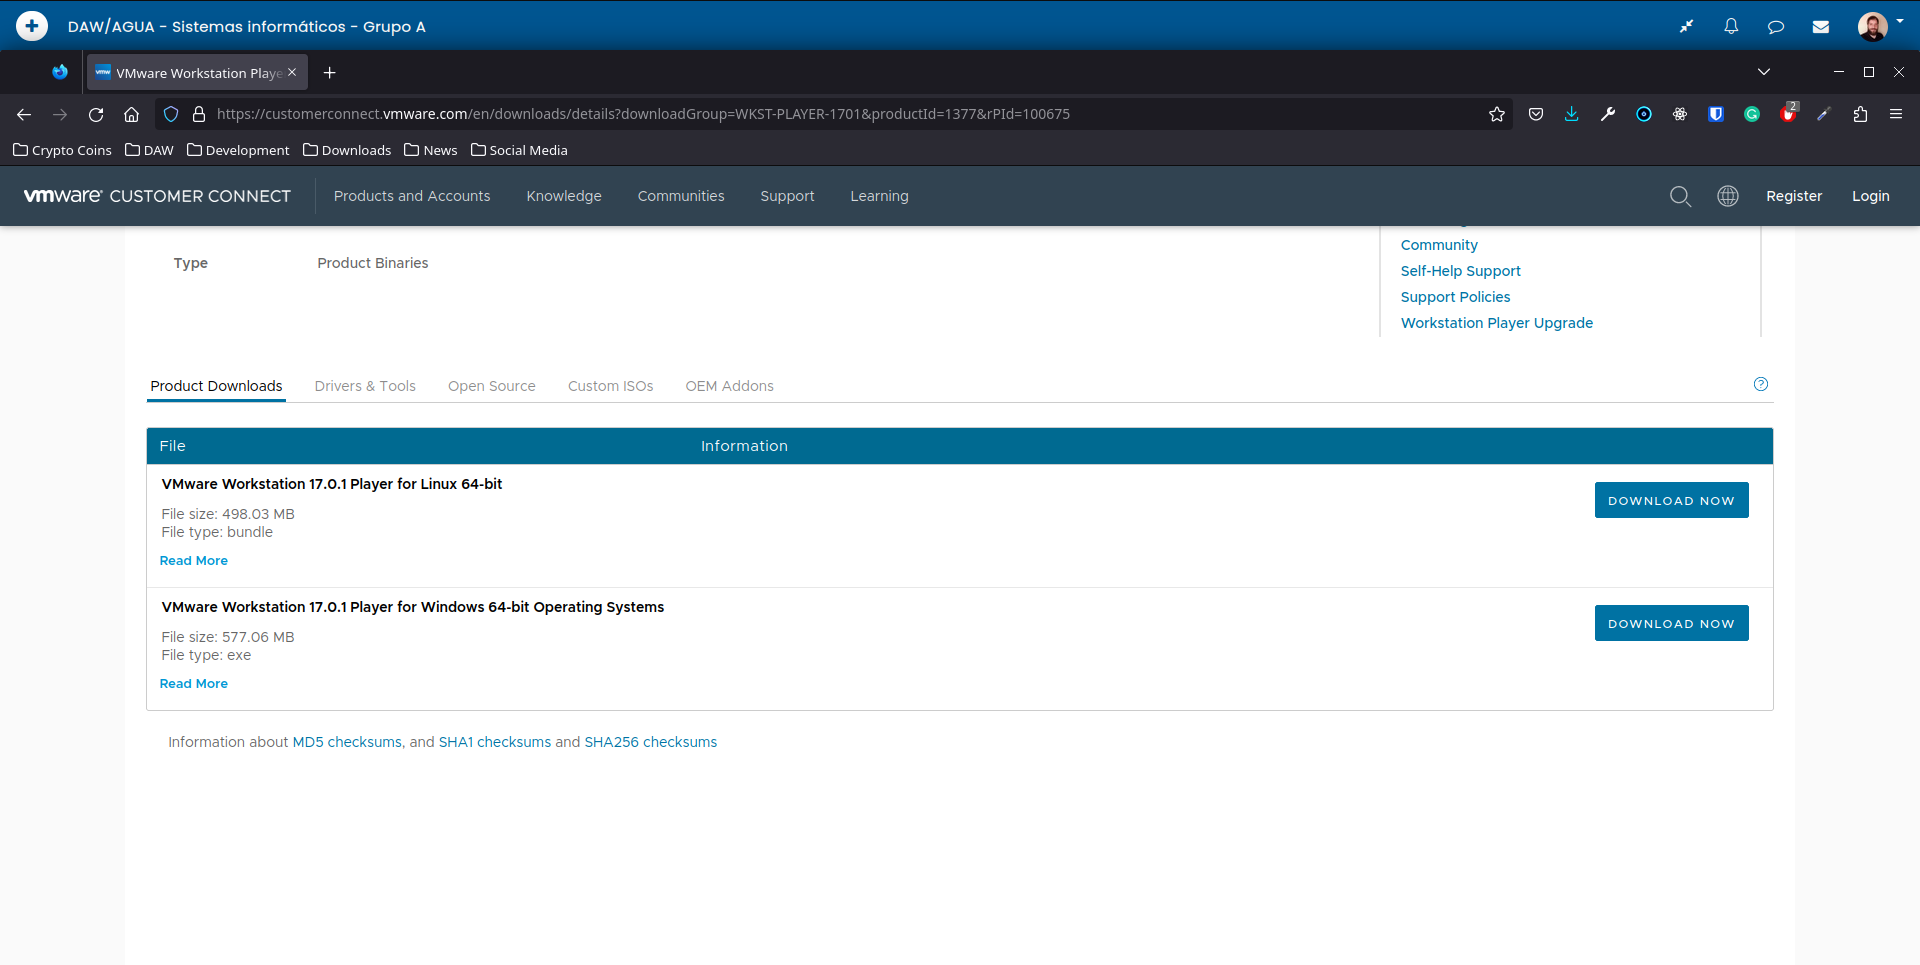
\includegraphics[scale=0.23]{vmware-download.png}
        \caption{Página de descarga de VMWare Workstation}
    \end{figure}

    \item A continuación hemos ejecutado el script que se nos ha proporcionado y que instalará el bundle de VMWare. En la siguiente captura se puede ver el script ejecutándose en una terminal y realizando la instalación de los paquetes.

    \begin{figure}[H]
        \centering
        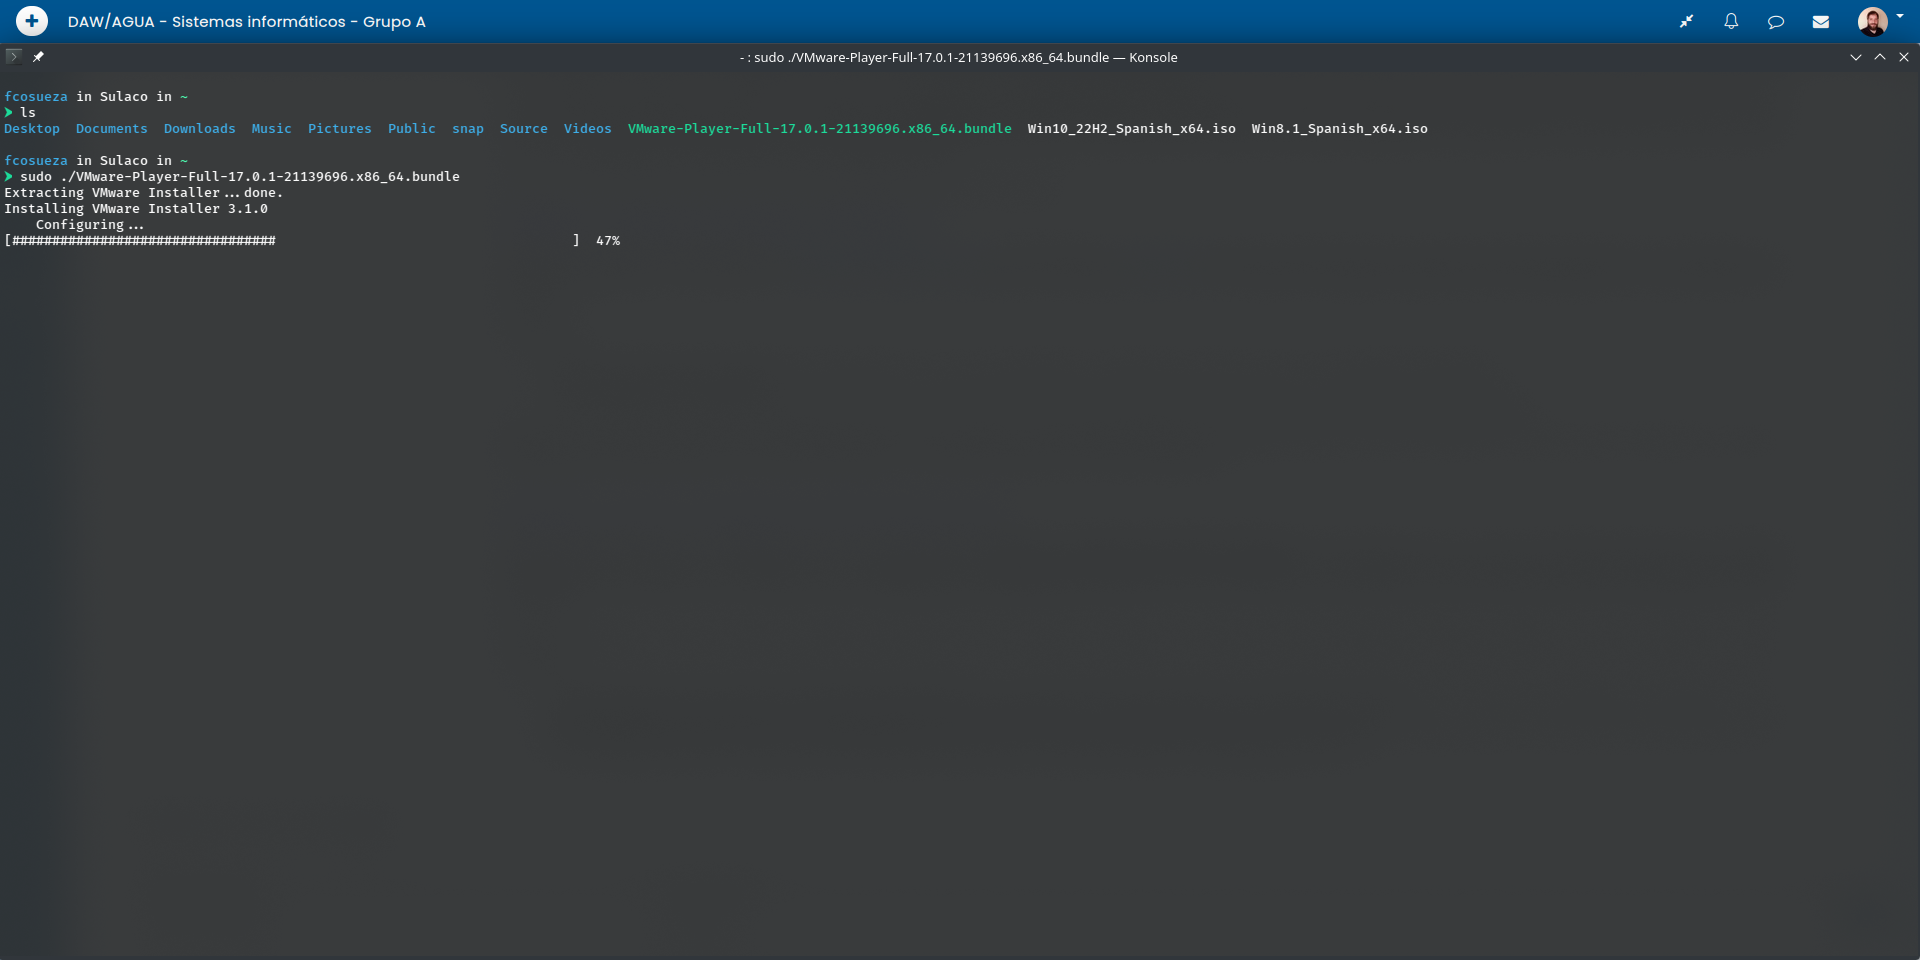
\includegraphics[scale=0.23]{vmware-install.png}
        \caption{Instalación de VMWare Workstation}
    \end{figure}

    \item Después de realizar la instalación desde la terminal y tras abrir por primera vez la aplicación, se nos da la opción de personalizar la instalación, aunque nosotros no hemos realizado ninguna modificación en esta. En la siguiente captura se muestra esta ventana.

    \begin{figure}[H]
        \centering
        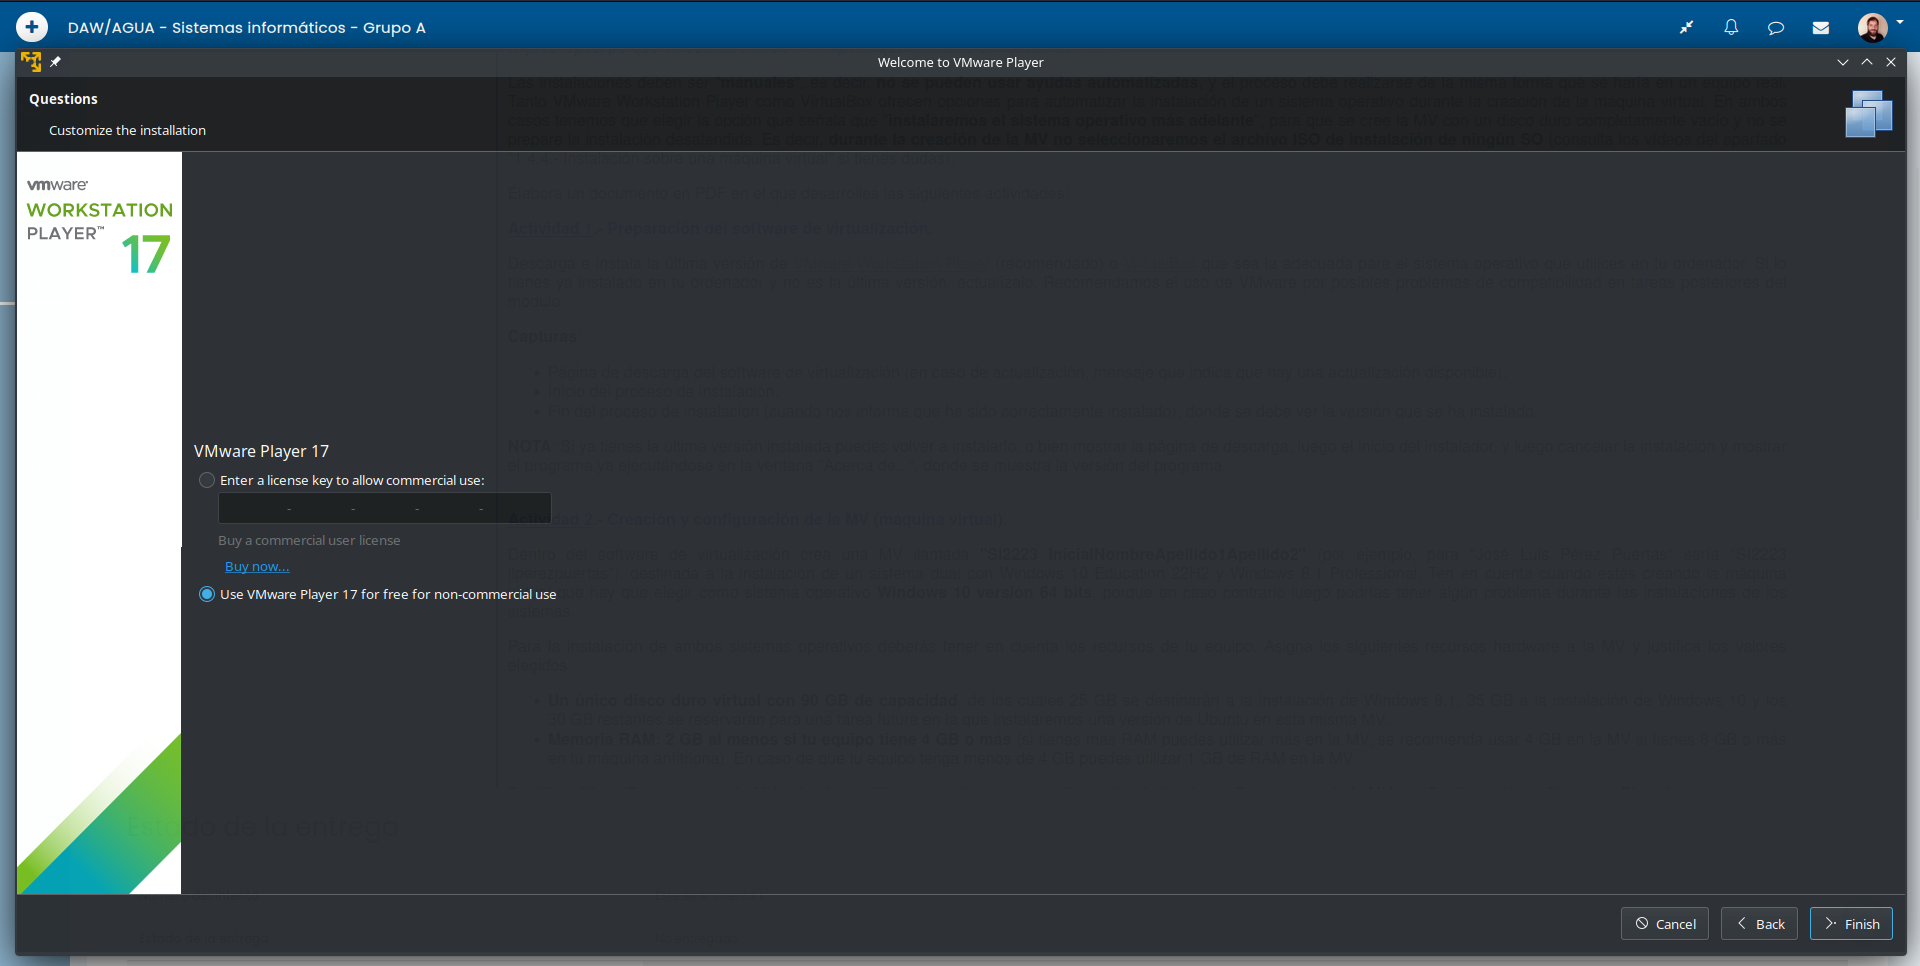
\includegraphics[scale=0.23]{vmware-install-2.png}
        \caption{Personalización de la Instalación de VMWare}
    \end{figure}

    \item Una vez llevado a cabo estos pasos, ya tenemos realizada la instalación de VMWare en Ubuntu. En la siguiente captura, podemos ver la máquina virtual instalada y sus especificaciones, así como la del host. Aunque en este portátil tengo 8 GB de RAM, la tarjeta gráfica no tiene memoria dedicada, por lo que 2 Gb de estos 8 están reservados para ese propósito, como muestra esta ventana, aunque ya hablaremos de esto en la siguiente sección.

    \begin{figure}[H]
        \centering
        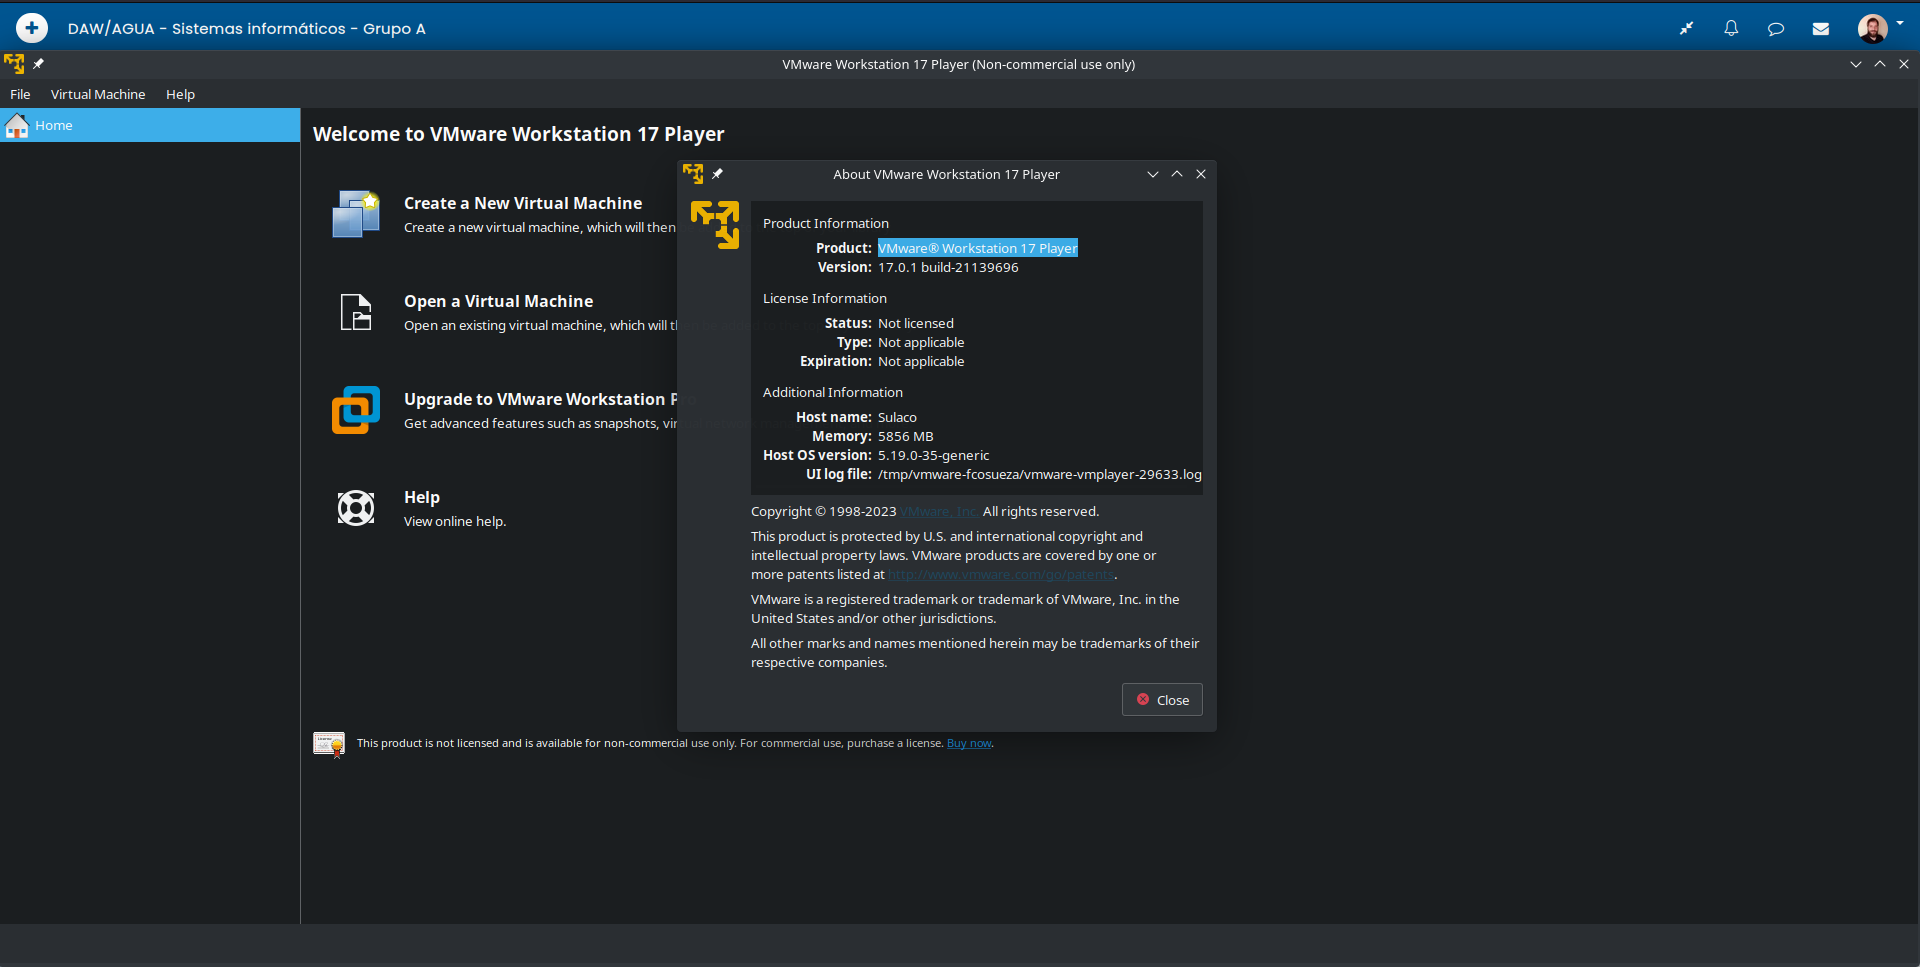
\includegraphics[scale=0.23]{vmware-install-3.png}
        \caption{Ventana de información sobre la versión instalada de VMWare}
    \end{figure}
\end{enumerate}

\subsection{Actividad 2: Creación y Configuración de la MV}

\subsection{Enunciado}
Dentro del software de virtualización crea una MV llamada ``SI2223 InicialNombreApellido1Apellido2'' (por ejemplo, para ``José Luis Pérez Puertas'' sería ``SI2223 jlperezpuertas''), destinada a la instalación de un sistema dual con Windows 10 Education 22H2 y Windows 8.1 Professional. Ten en cuenta cuando estés creando la máquina virtual que hay que elegir como sistema operativo Windows 10 versión 64 bits, porque en caso contrario luego podrías tener algún problema durante las instalaciones de los sistemas.

Para la instalación de ambos sistemas operativos deberás tener en cuenta los recursos de tu equipo. Asigna los siguientes recursos hardware a la MV y justifica los valores elegidos:

\begin{itemize}
    \item \textbf{Un único disco duro virtual con 90 GB de capacidad}, de los cuales 25 GB se destinarán a la instalación de Windows 8.1, 35 GB a la instalación de Windows 10 y los 30 GB restantes se reservarán para una tarea futura en la que instalaremos una versión de Ubuntu en esta misma MV.

    \item \textbf{Memoria RAM: 2 GB al menos si tu equipo tiene 4 GB o más}, (si tienes más RAM puedes utilizar más en la MV, se recomienda usar 4 GB en la MV si tienes 8 GB o más en tu máquina anfitriona). En caso de que tu equipo tenga menos de 4 GB puedes utilizar 1 GB de RAM en la MV.
\end{itemize}


Si utilizas VirtualBox, tras crear la MV deberás modificar un parámetro de configuración de la misma. Entra dentro de la MV en ``Configuración > Sistema > Placa base'' y marca la opción ``Habilitar EFI''. Esto hará que la MV utilice un firmware de tipo UEFI, tal como es común en los equipos reales actuales.

\textbf{Capturas}

\begin{itemize}
    \item Introducción del nombre de la máquina y elección de tipo ``Windows 10 64 bits''.
    \item Cantidad de RAM asignada.
    \item Tamaño de disco duro asignado.
    \item Resumen con los datos de la máquina virtual creada en la ventana principal del programa de virtualización (en VirtualBox se debe ver en ``Sistema'' la opción ``EFI: Habilitado'').
\end{itemize}

\subsubsection{Solución}
En este apartado vamos a realizar la creación y configuración de la máquina virtual con las especificaciones pedidas en el enunciado. Para ello, se han llevado a cabo lo siguientes pasos:

\begin{enumerate}
    \item En primer lugar hemos pulsado la opción ``\textbf{Create new virtual machine}'' que nos ha abierto un menú donde se nos da la opción de instalar directamente el sistema operativo guest, ya sea desde un cd-rom o una imagen ISO, o dejar la instalación para más tarde, que es lo que hemos elegido ya que nosotros vamos a realizar la instalación de forma manual.

    \begin{figure}[H]
        \centering
        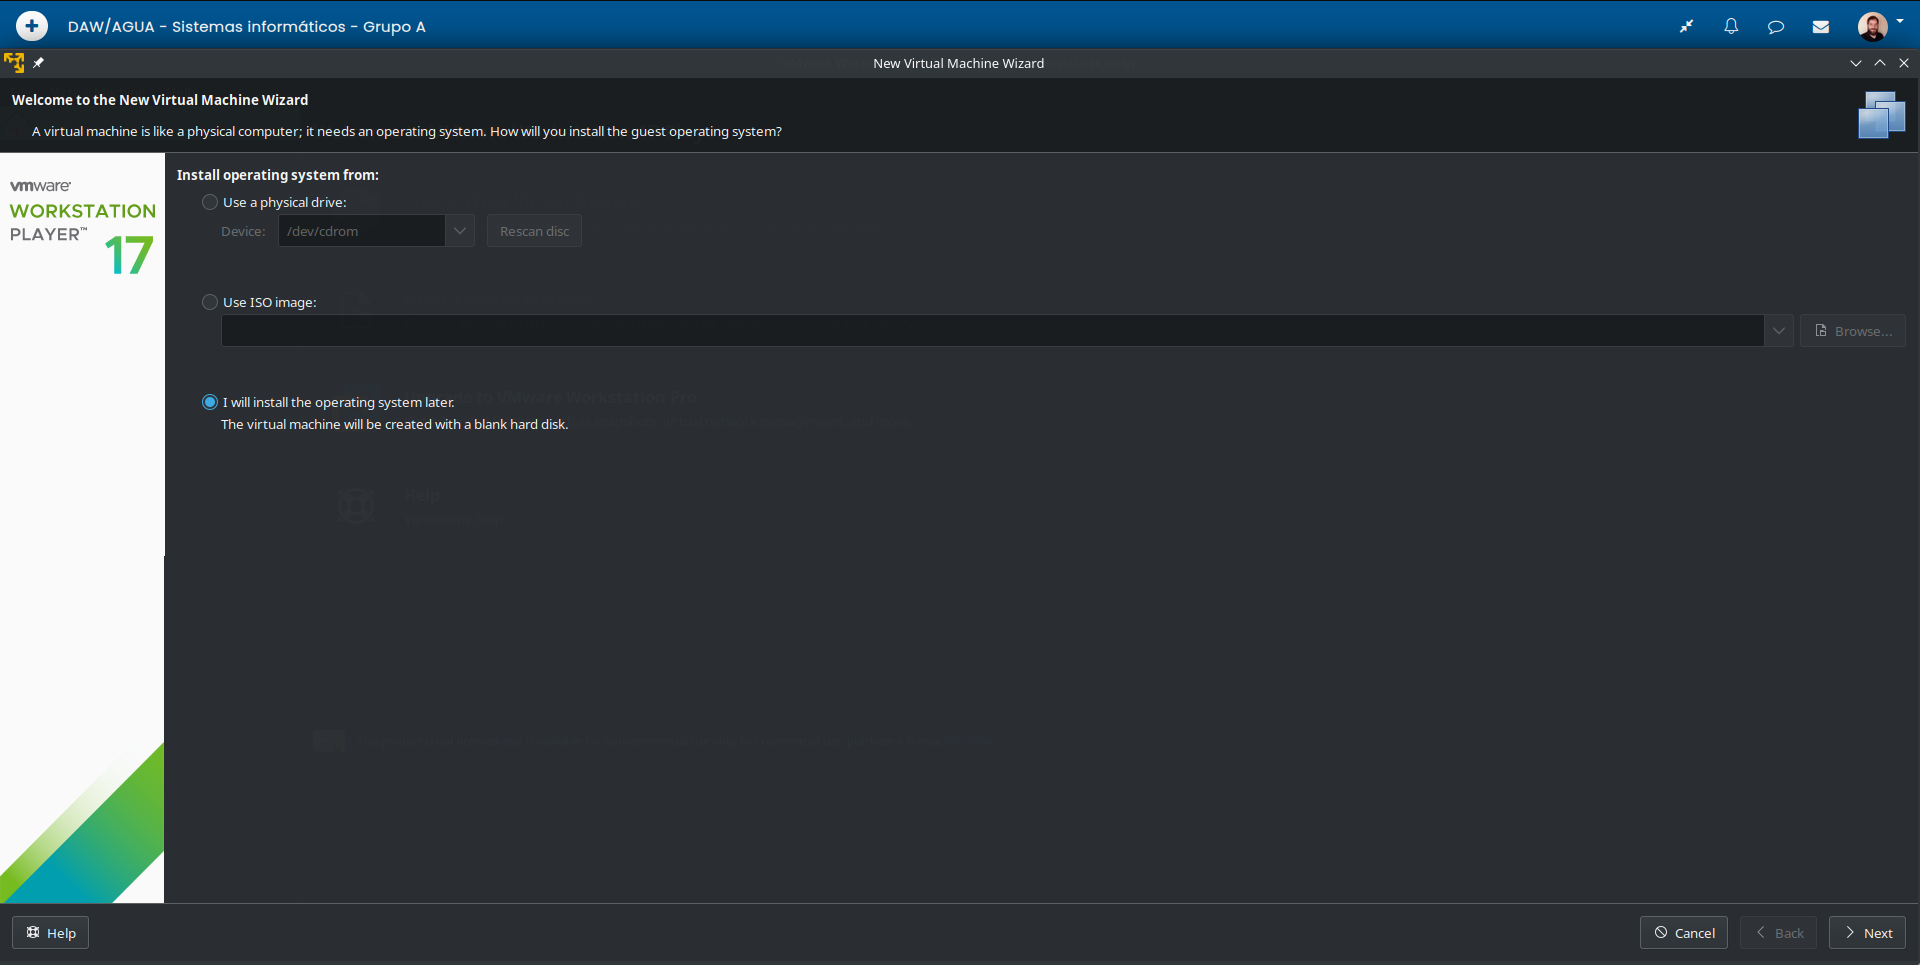
\includegraphics[scale=0.23]{vmware-create-1.png}
        \caption{Selección del modo de instalación del SO en la máquina virtual}
    \end{figure}

    \item En la siguiente pantalla se nos da la opción de seleccionar el \textbf{tipo de sistema operativo} que vamos a instalar en la máquina virtual. Nosotros hemos seleccionado ``\textit{Windows 10 x64}'', tal y como se nos pide en el enunciado, como podemos ver en la siguiente captura.

    \begin{figure}[H]
        \centering
        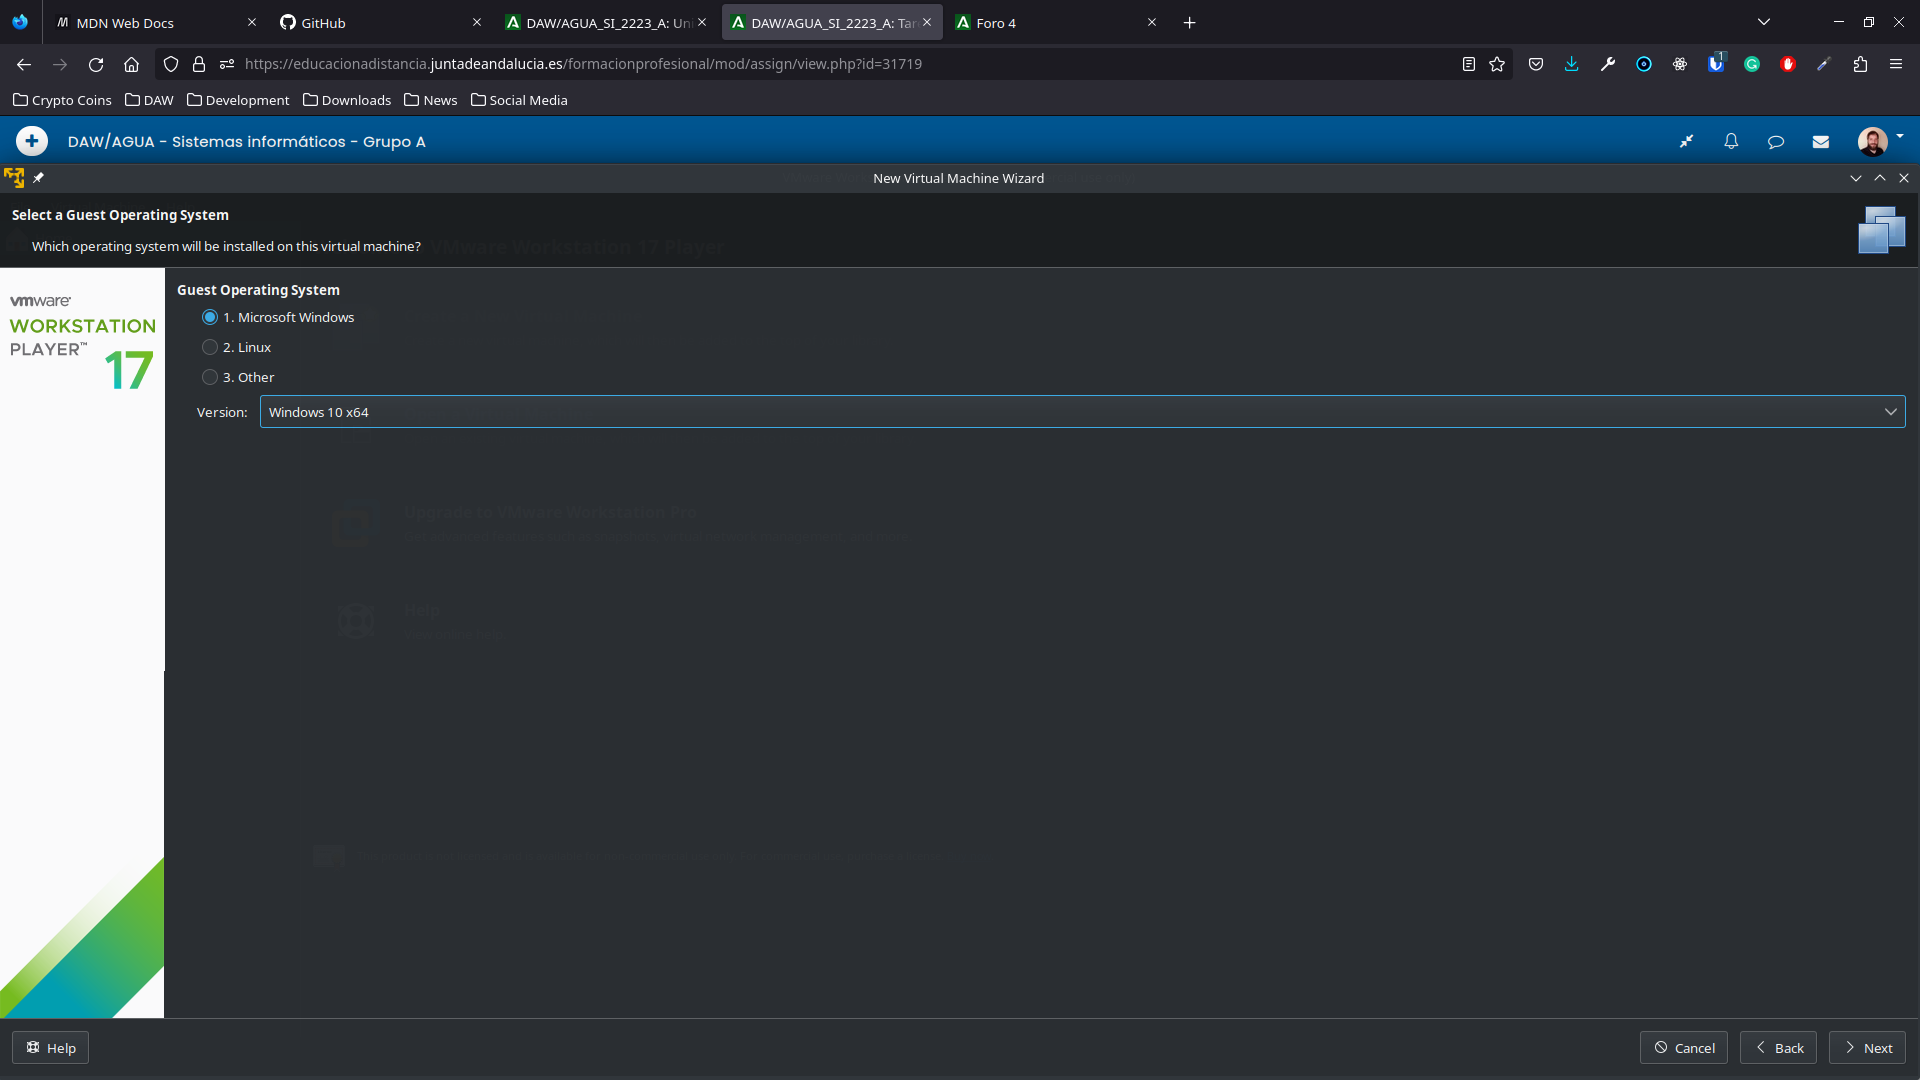
\includegraphics[scale=0.23]{vmware-create-2.png}
        \caption{Selección del tipo de sistema operativo en la creación de la máquina virtual}
    \end{figure}

    \item Tras pulsar en \textit{next}, se nos muestra una pantalla que nos permite \textbf{introducir el nombre de la máquina virtual} que se va a crear. En nuestro caso, el nombre que se ha introducido ha sido \textbf{SI2223 fjsuezarodriguez}, siguiendo el patrón que se nos indica en el enunciado del problema.

    \begin{figure}[H]
        \centering
        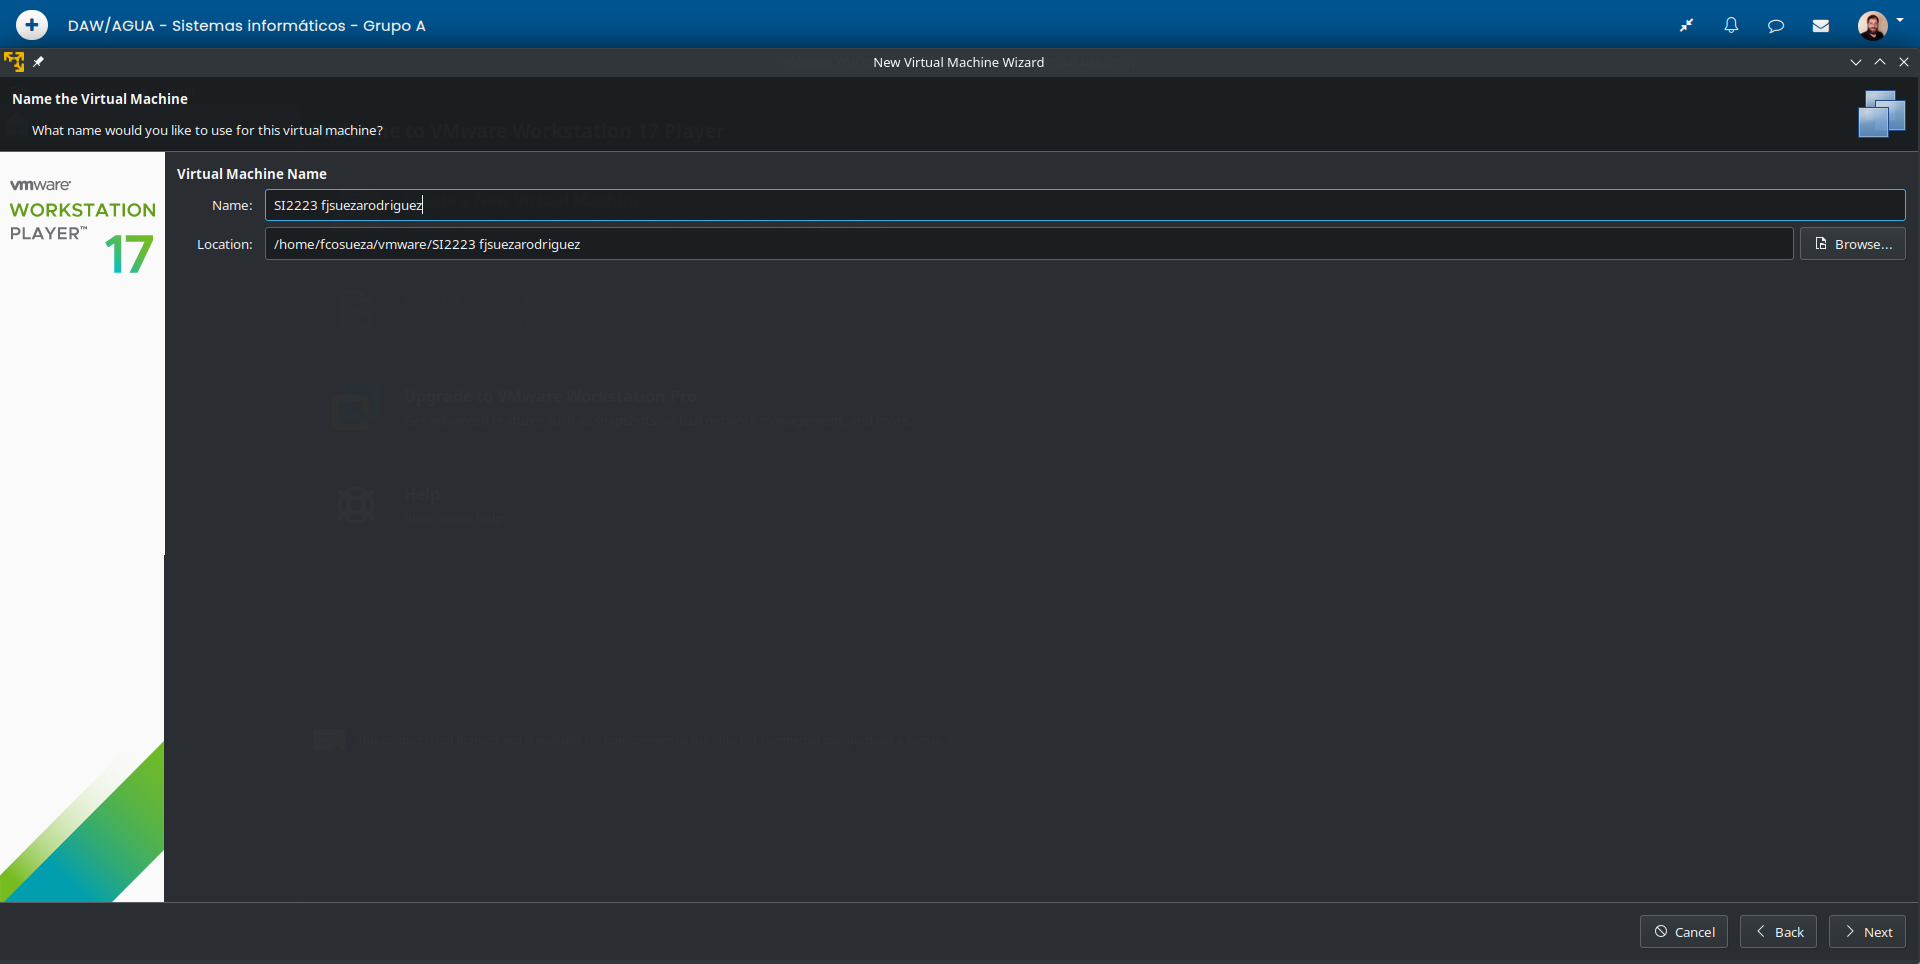
\includegraphics[scale=0.23]{vmware-create-3.png}
        \caption{Introducción del nombre de la máquina virtual a crear}
    \end{figure}

    \item Una vez establecido el nombre de la máquina virtual, se nos pide que introduzcamos el \textbf{espacio de disco duro} que vamos a reservar para esta. Por defecto se reservan 60 GB, pero nosotros hemos aumentado esa cantidad a 90 GB ya que tenemos pensado instalar varios sistemas operativos.

    \begin{figure}[H]
        \centering
        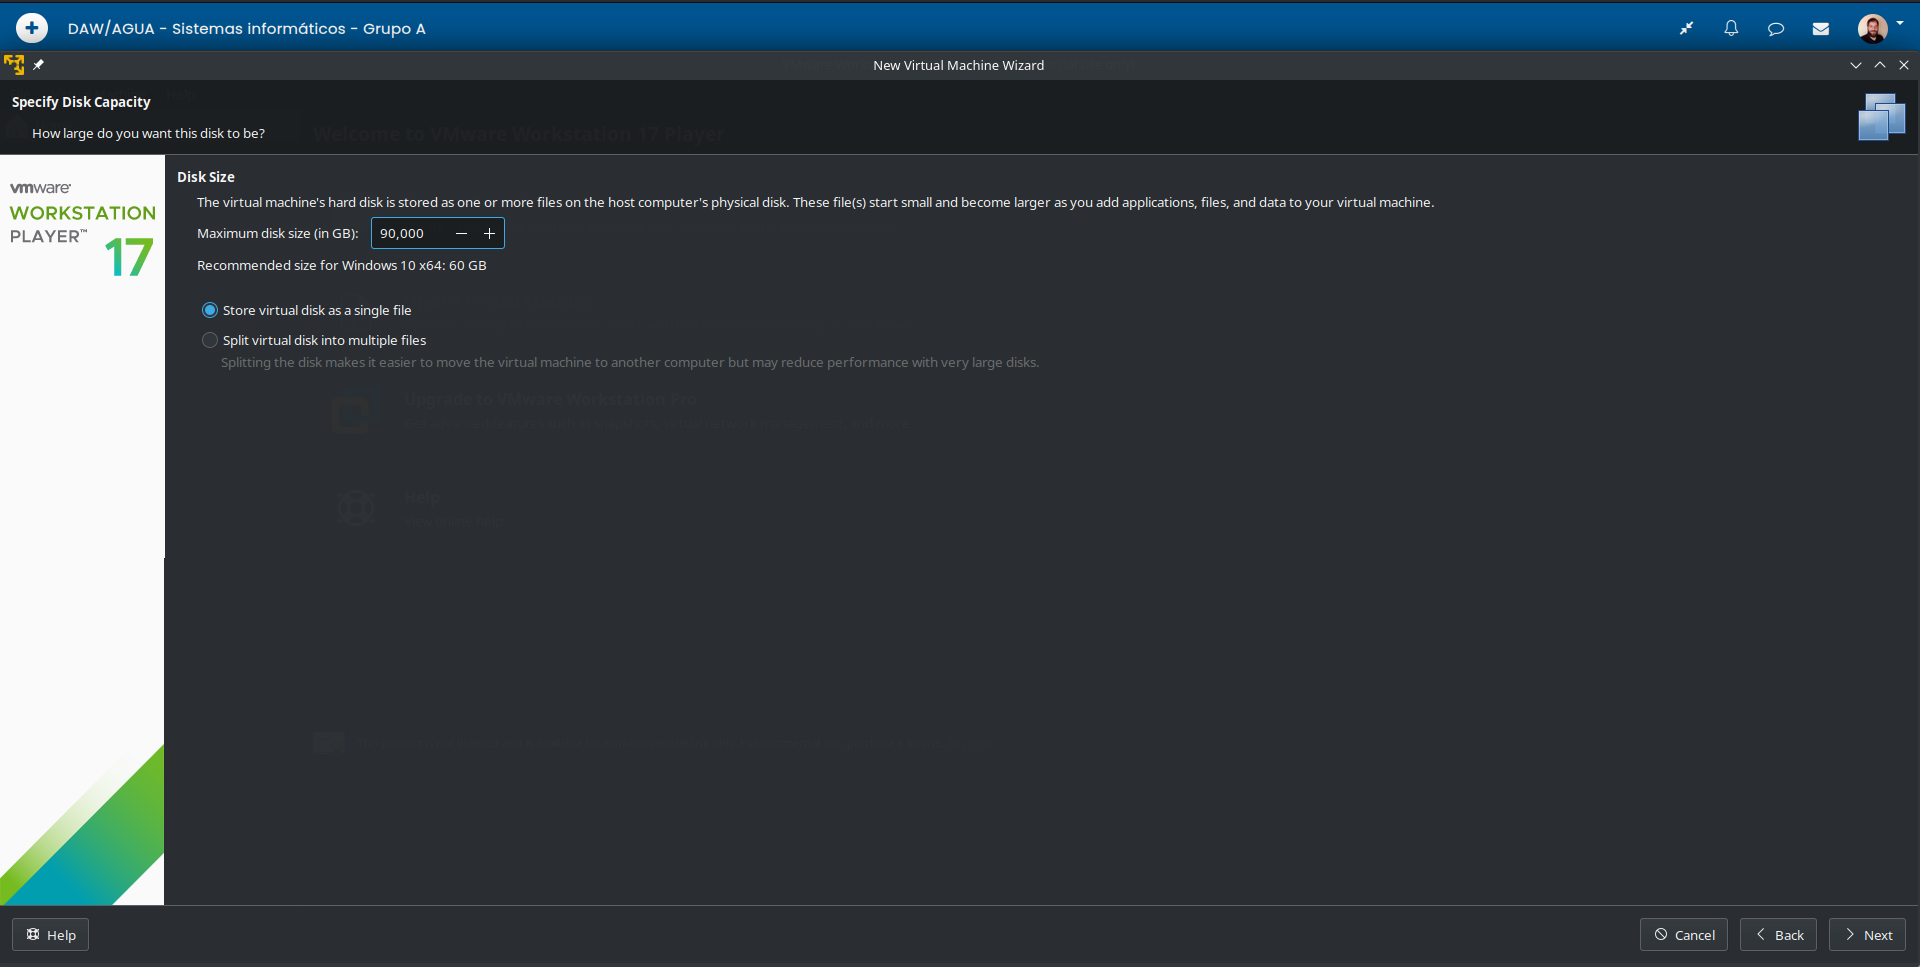
\includegraphics[scale=0.23]{vmware-create-4.png}
        \caption{Reserva de espacio de disco duro para la máquina virtual}
    \end{figure}

    \item Tras el último paso, y después de pulsar en next, se nos muestra un \textbf{resumen con las características de la máquina virtual} que se va a crear. En nuestro caso no se nos ha pedido que cambiemos o seleccionemos la cantidad de memoria RAM que será usada para esta máquina. Por defecto, el sistema ha \textbf{reservado 2 GB de memoria RAM}, que es la cantidad de queríamos reservar.

    Se va a reservar esta cantidad porque aunque el \textbf{sistema anfitrión} tiene \textbf{8 GB de memoria RAM}, tiene una \textbf{tarjeta de vídeo integrada sin memoria dedicada}, en concreto una AMD Vega 8, por lo que de estos 8 GB, 2 GB se reservan para esta tarjeta, así que \textbf{contamos con 6 GB de RAM} para el sistema. Para que no tengamos problemas y el sistema anfitrión pueda sufrir ralentizaciones, y teniendo en cuenta que con 2 GB los sistemas visitantes que vamos a instalar pueden funcionar perfectamente, vamos a elegir esta cantidad.

    En la siguiente captura vemos la información mostrada en esta ventana resumiendo las características de la máquina virtual a crear.

    \begin{figure}[H]
        \centering
        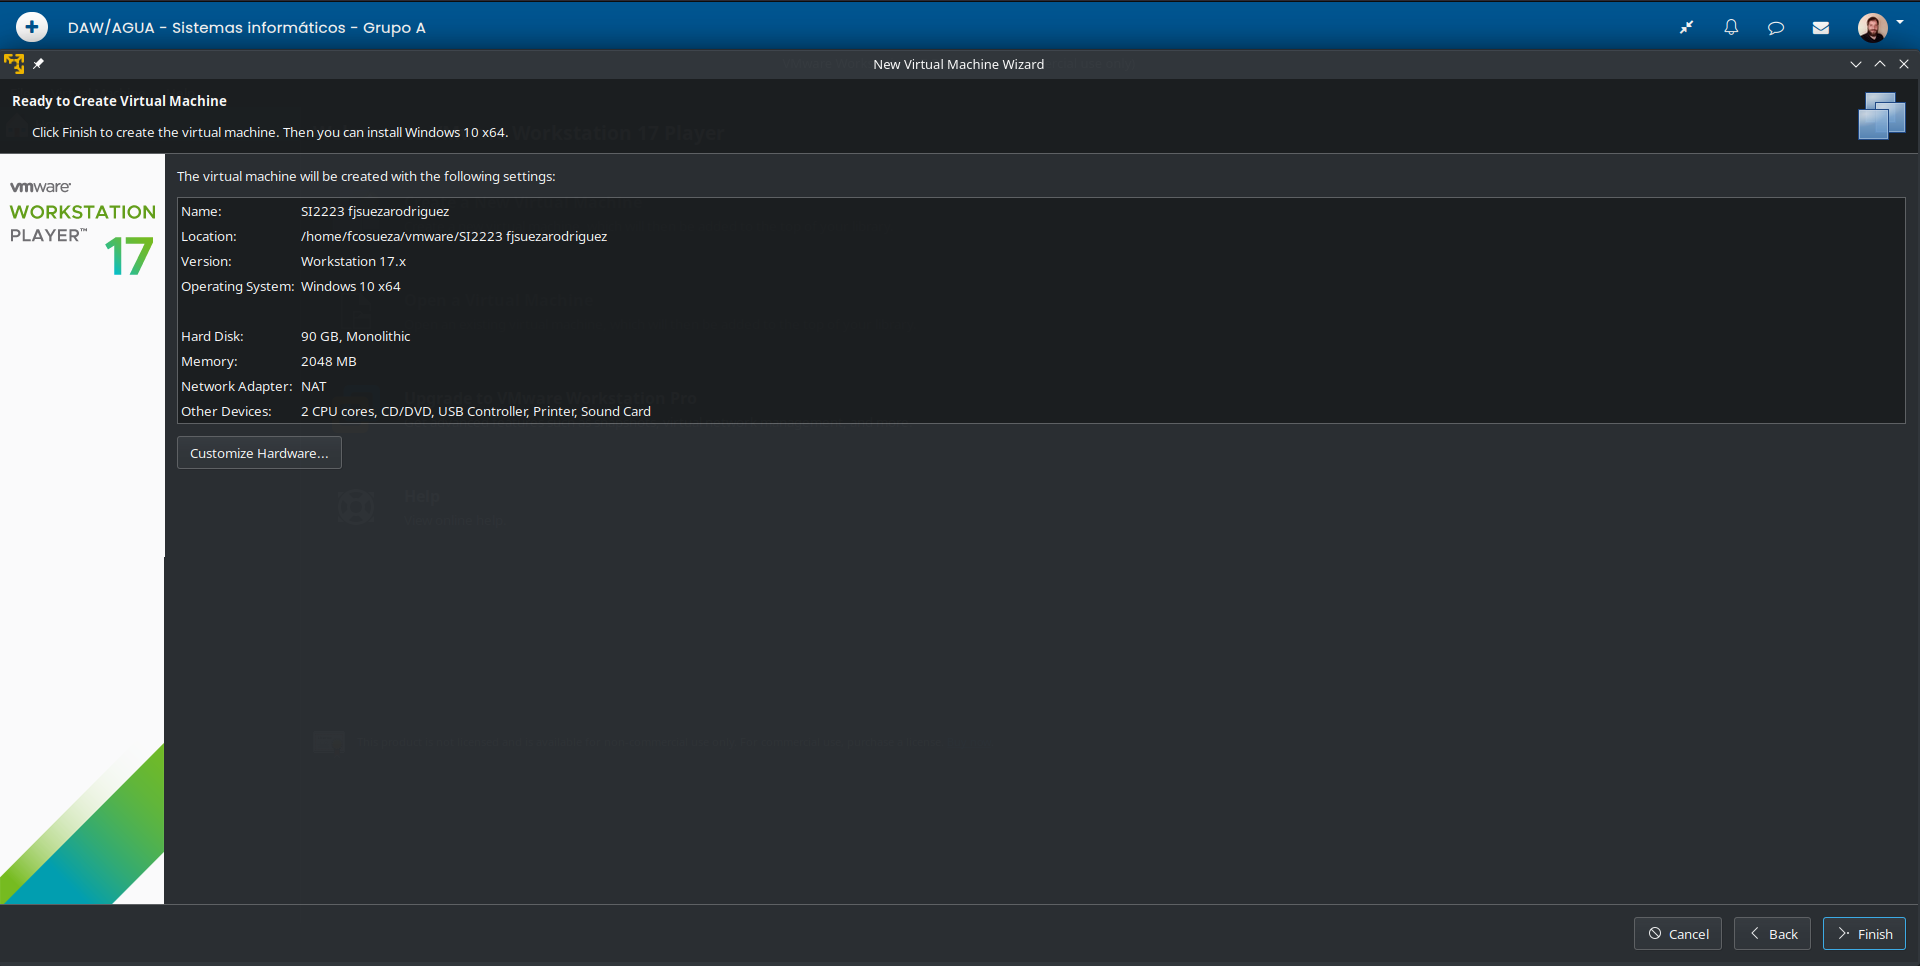
\includegraphics[scale=0.23]{vmware-create-5.png}
        \caption{Información sobre la máquina virtual que se va a crear}
    \end{figure}

    Aún así, si la cantidad de RAM reservada no se ajustara a lo que nosotros queremos, podemos pulsar en la opción ``\textbf{Customize Hardware}'' donde se nos abrirá una donde podemos cambiar cualquier de las características de la máquina virtual, como se ve en la siguiente captura.

    \begin{figure}[H]
        \centering
        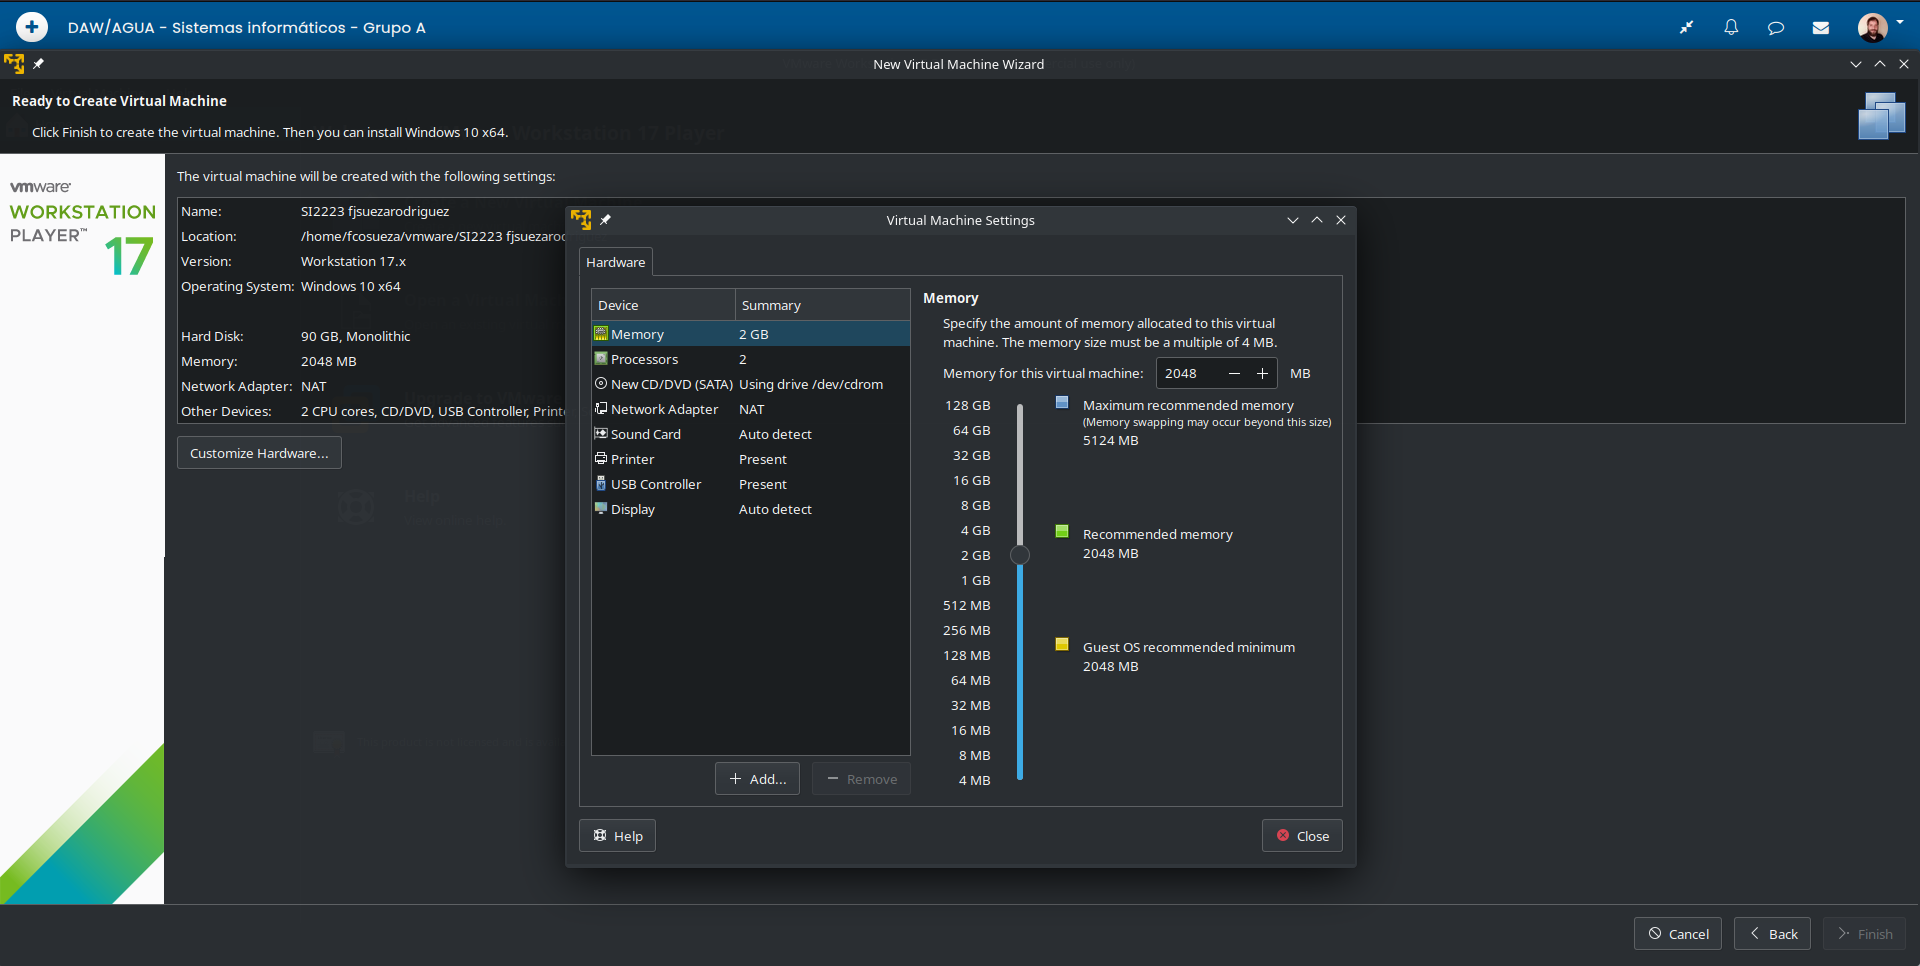
\includegraphics[scale=0.23]{vmware-create-6.png}
        \caption{Personalización de las características de la MV}
    \end{figure}

    \item Por último, mostramos la información relativa a la máquina virtual ya creada en la ventana principal de VMWare. No se nos muestra información muy detallada, pero si pulsamos en ``\textbf{Edit virtual machine settings}'', se nos abrirá una ventana con información mas detallada y que podemos también cambiar.

    \textbf{NOTA}: en este punto solo se incluye la captura de la información de la máquina virtual en la página principal de VMWare. No se incluye la ventana con la información más detallada ya que es la misma que se muestra en la Figura 2.10, por lo que para no repetir capturas, solo se incluye la especificada.

    \begin{figure}[H]
        \centering
        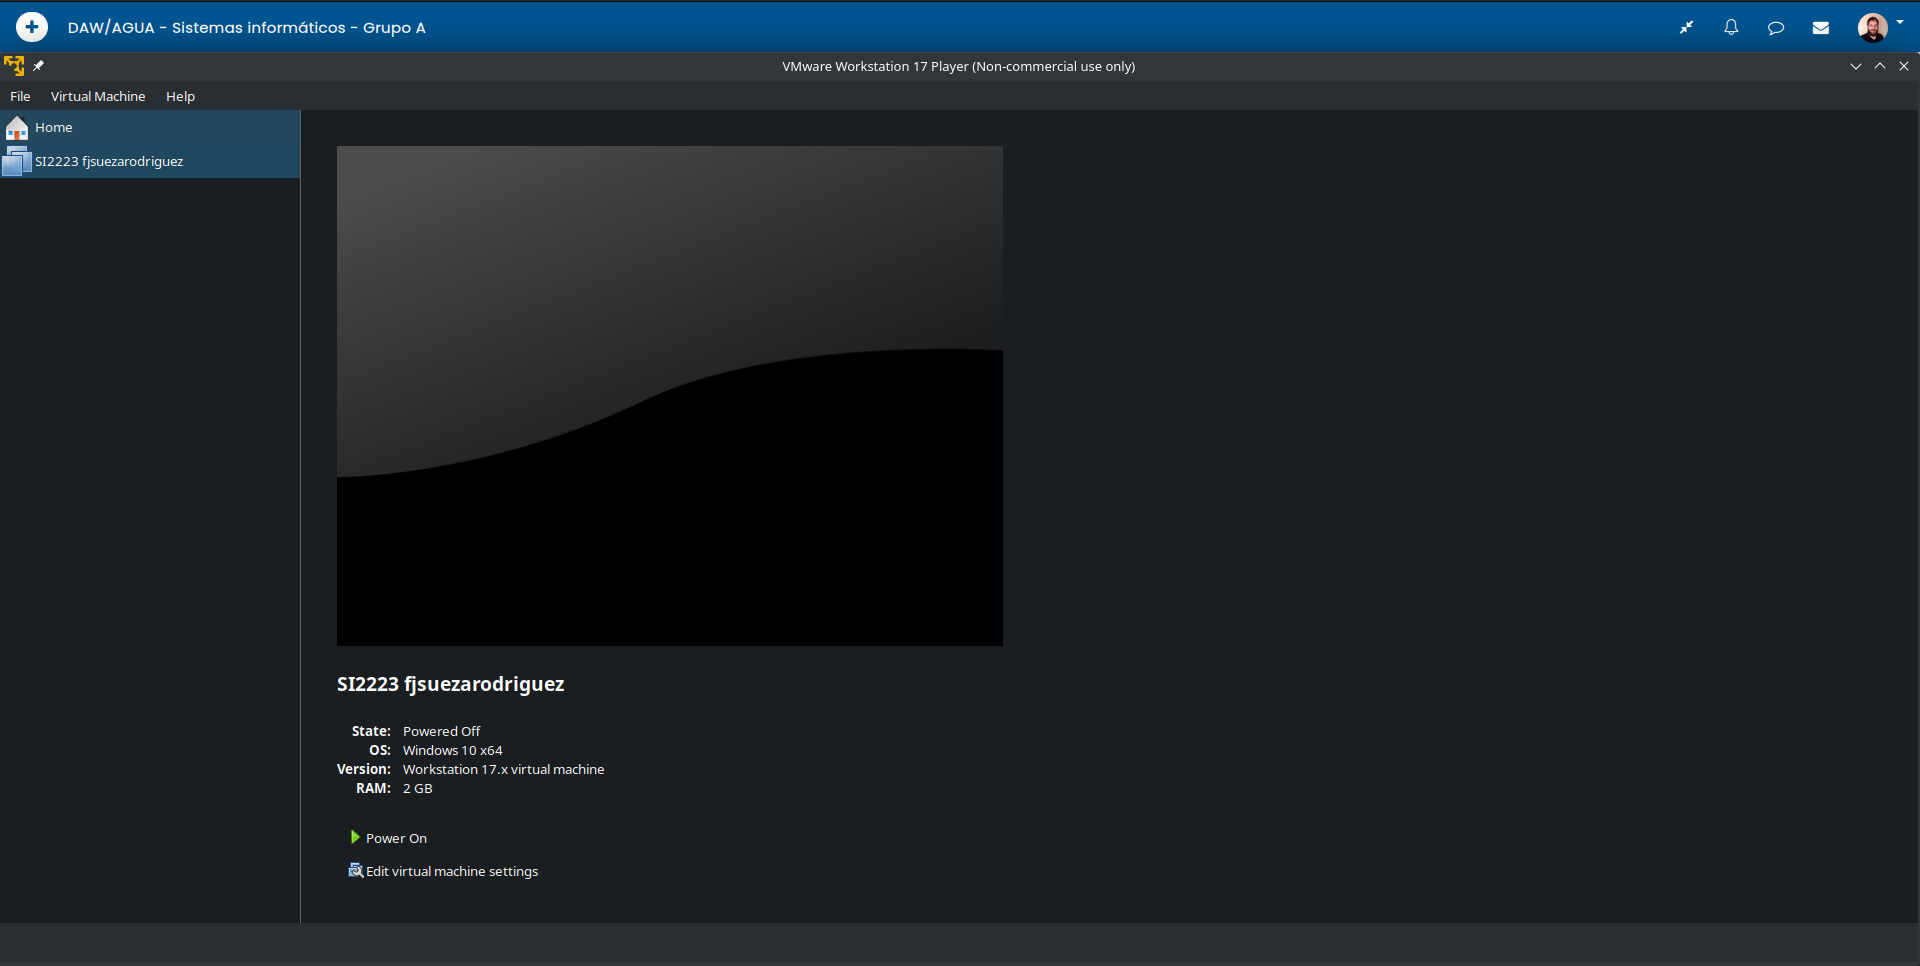
\includegraphics[scale=0.23]{vmware-create-7.png}
        \caption{Información de la MV creada en la ventana principal de VMWare}
    \end{figure}
\end{enumerate}

\subsection{Actividad 3: Instalación de Windows 8.1 Professional}
Instala primero Windows 8.1 Professional en la MV, pero ten en cuenta que durante su instalación tendrás que realizar operaciones relativas al particionado del disco duro virtual para asegurar que dejas espacio disponible para las futuras instalaciones de Windows 10 y Ubuntu. Durante el particionado, crea una partición de 25 GB, y Windows creará algunas otras particiones de manera automática. Deberás describir cada una de las particiones creadas durante este proceso.

Durante la instalación define un usuario local (sin cuenta de Microsoft) cuyo nombre sea la primera letra de tu nombre seguido de tus apellidos completos, por ejemplo, para \textbf{José Luis Pérez Puertas} el usuario debería ser \textbf{\textbf{jlperezpuertas}}. Respecto a la clave de este usuario ponle \textbf{admin2223}.

\textbf{Capturas}:

\begin{itemize}
    \item Elección del archivo ISO de instalación del sistema.
    \item Inicio del proceso de instalación.
    \item Introducción de la clave de activación.
    \item Esquema de particionado en el que se ven todas las particiones que se han creado (antes de comenzar con la copia de archivos). Recuerda acompañar esta captura con una descripción de cada una de las particiones que se hayan creado.
    \item Creación del usuario y establecimiento de la contraseña.
    \item Muestra de que el sistema ha sido debidamente instalado.
\end{itemize}

\subsubsection{Solución}
En este ejercicio vamos a realizar la instalación de Windows 8.1 Professional. Para llevarla a cabo, vamos a seguir los siguientes pasos:

\begin{enumerate}
    \item Para empezar, vamos a iniciar la máquina virtual que creamos en los apartados anteriores, y desde la opción ``\textbf{Virtual Machine -> Removable Devices}'' vamos a seleccionar la imagen de Windows 8.1 Professional que hemos descargado previamente. Una vez realizado esto, deberemos reiniciar la máquina virtual y pulsar alguna tecla, como se nos indica, para inicializar la instalación de Windows.

    \begin{figure}[H]
        \centering
        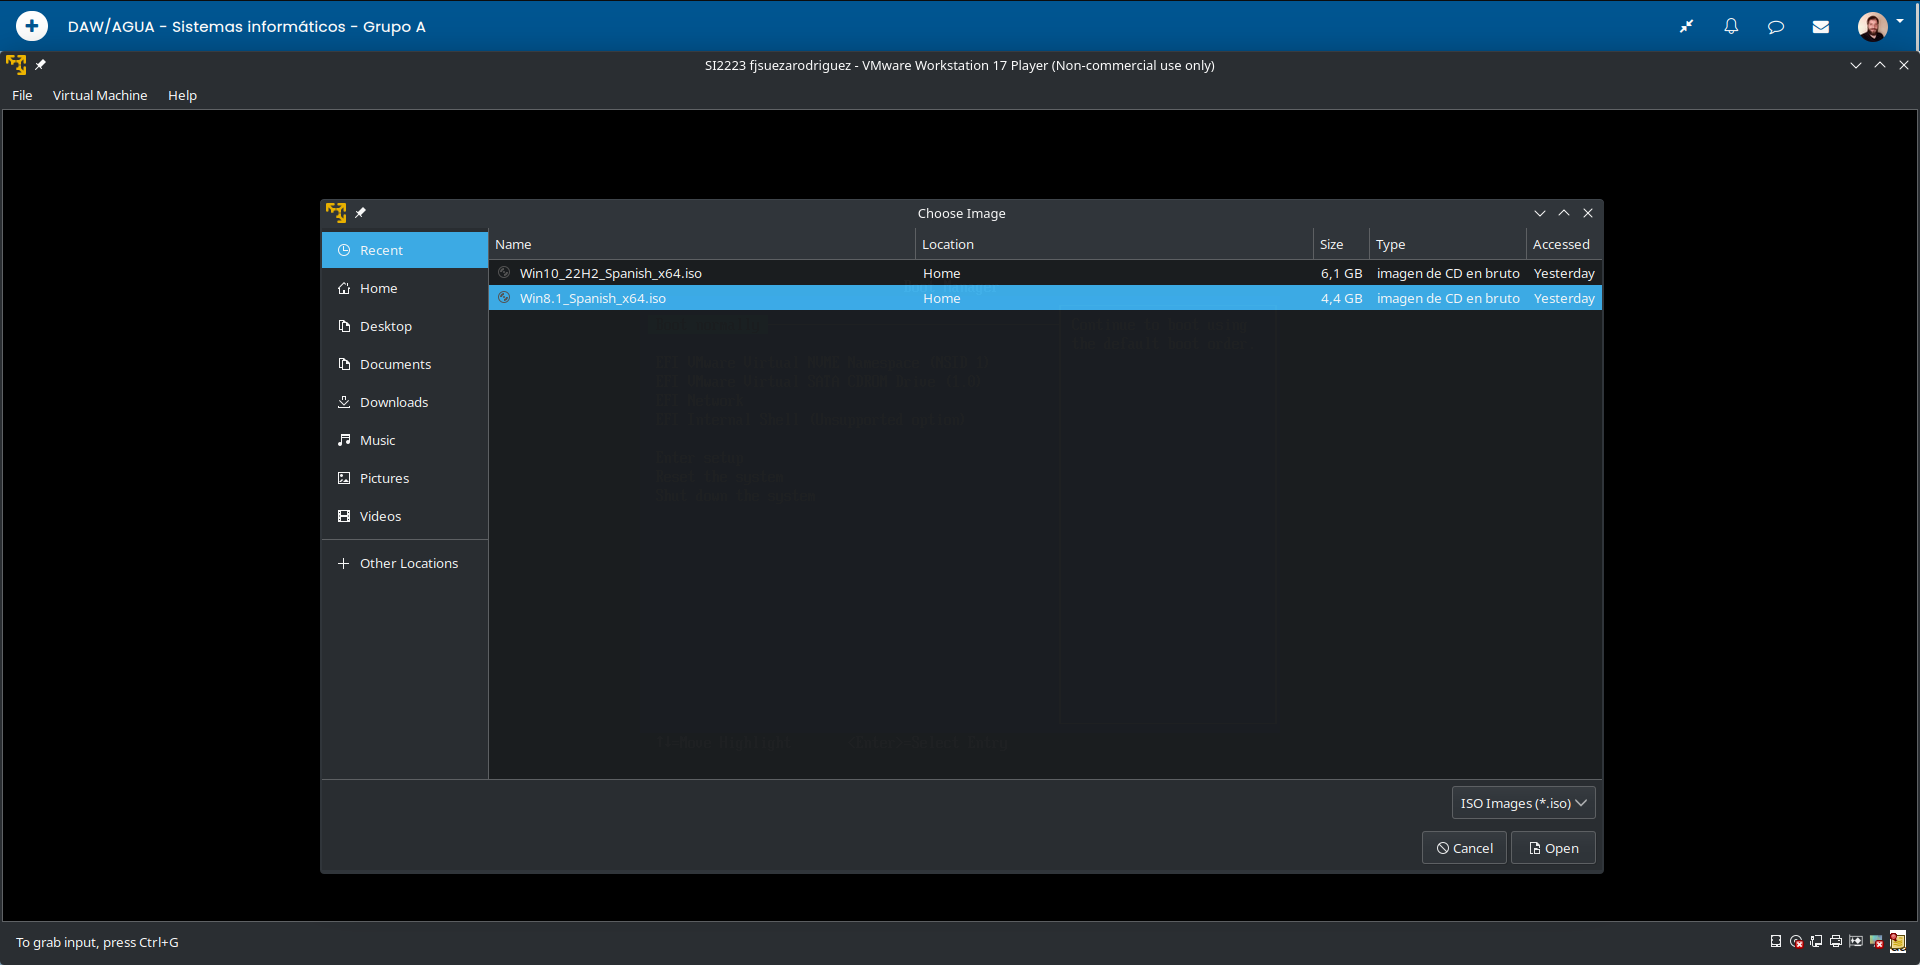
\includegraphics[scale=0.23]{windows8-install-1.png}
        \caption{Selección de la imagen ISO de Windows 8.1}
    \end{figure}

    \item Una vez cargada la imagen, nos aparecerá una pantalla para seleccionar el idioma de la instalación, así como la versión de Windows a instalar. Una vez seleccionada, podremos comenzar el proceso de instalación pulsando en la pantalla que se nos mostrará a continuación.

    \begin{figure}[H]
        \centering
        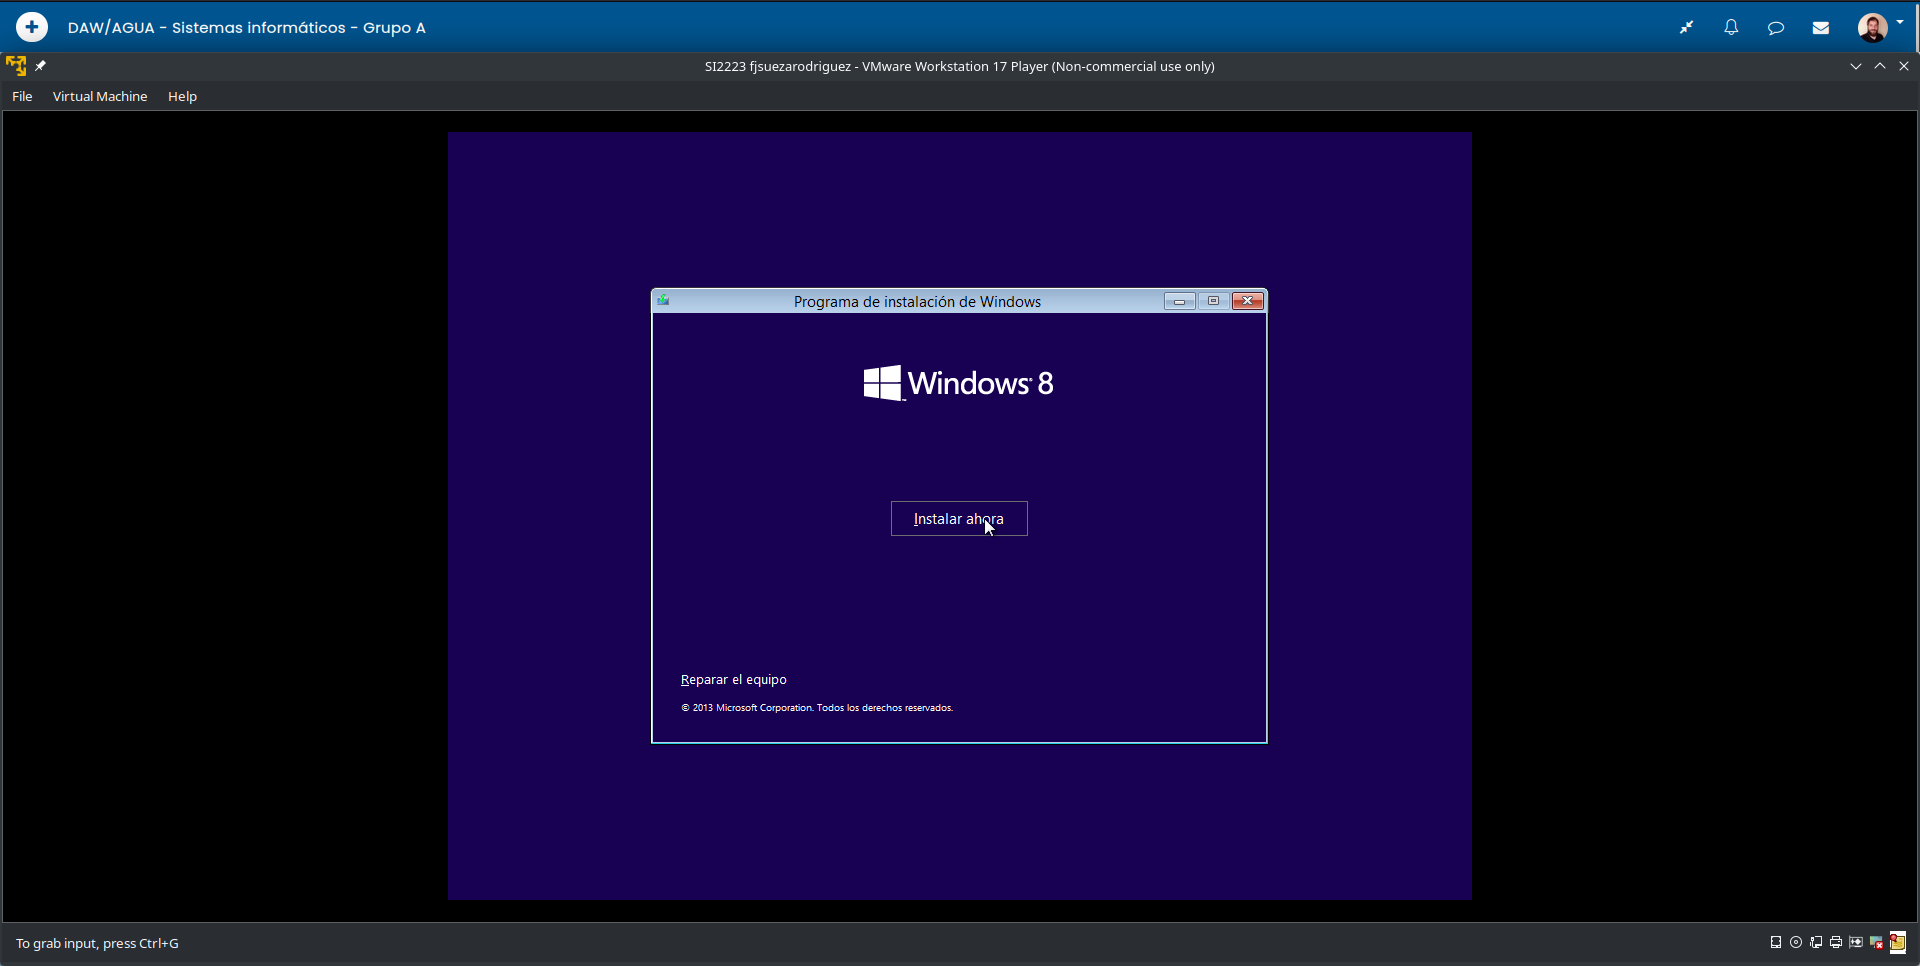
\includegraphics[scale=0.23]{windows8-install-2.png}
        \caption{Pantalla de inicio de instalación de Windows 8.1}
    \end{figure}

    Como vemos en la parte inferior izquierda, también se nos da la opción ``\textbf{Reparar el Sistema}'', en caso de que ya tengamos Windows instalado y queramos repararlo, aunque esta opción no se va a discutir en este documento.

    \item Una vez inicializada la instalación, lo primero que se nos pedirá es que introduzcamos la \textbf{clave de producto} de Windows 8.1. Esta clave, sirve para activar Windows y evitar que se use el software de forma ilegal.

    Podemos encontrar diferentes \textbf{licencias retail} en la página de \textbf{Microsoft Store}, siendo su precio bastante alto. En internet encontraremos \textbf{decenas de webs} donde también se puede adquirir licencias de Microsoft Windows a precios muy asequibles, pero estas \textbf{licencias son ilegales}, ya que la mayoría son \textbf{licencias de tipo OEM} que solo pueden usar los fabricantes y quedan ligadas al hardware donde se instalan, por lo que usarlas en otros dispositivos, y más aun venderlas, incumple la EULA de Microsoft, por lo que hay que tener cuidado donde adquirimos nuestra licencia, y procurar hacerlo en tiendas autorizadas.

    \begin{figure}[H]
        \centering
        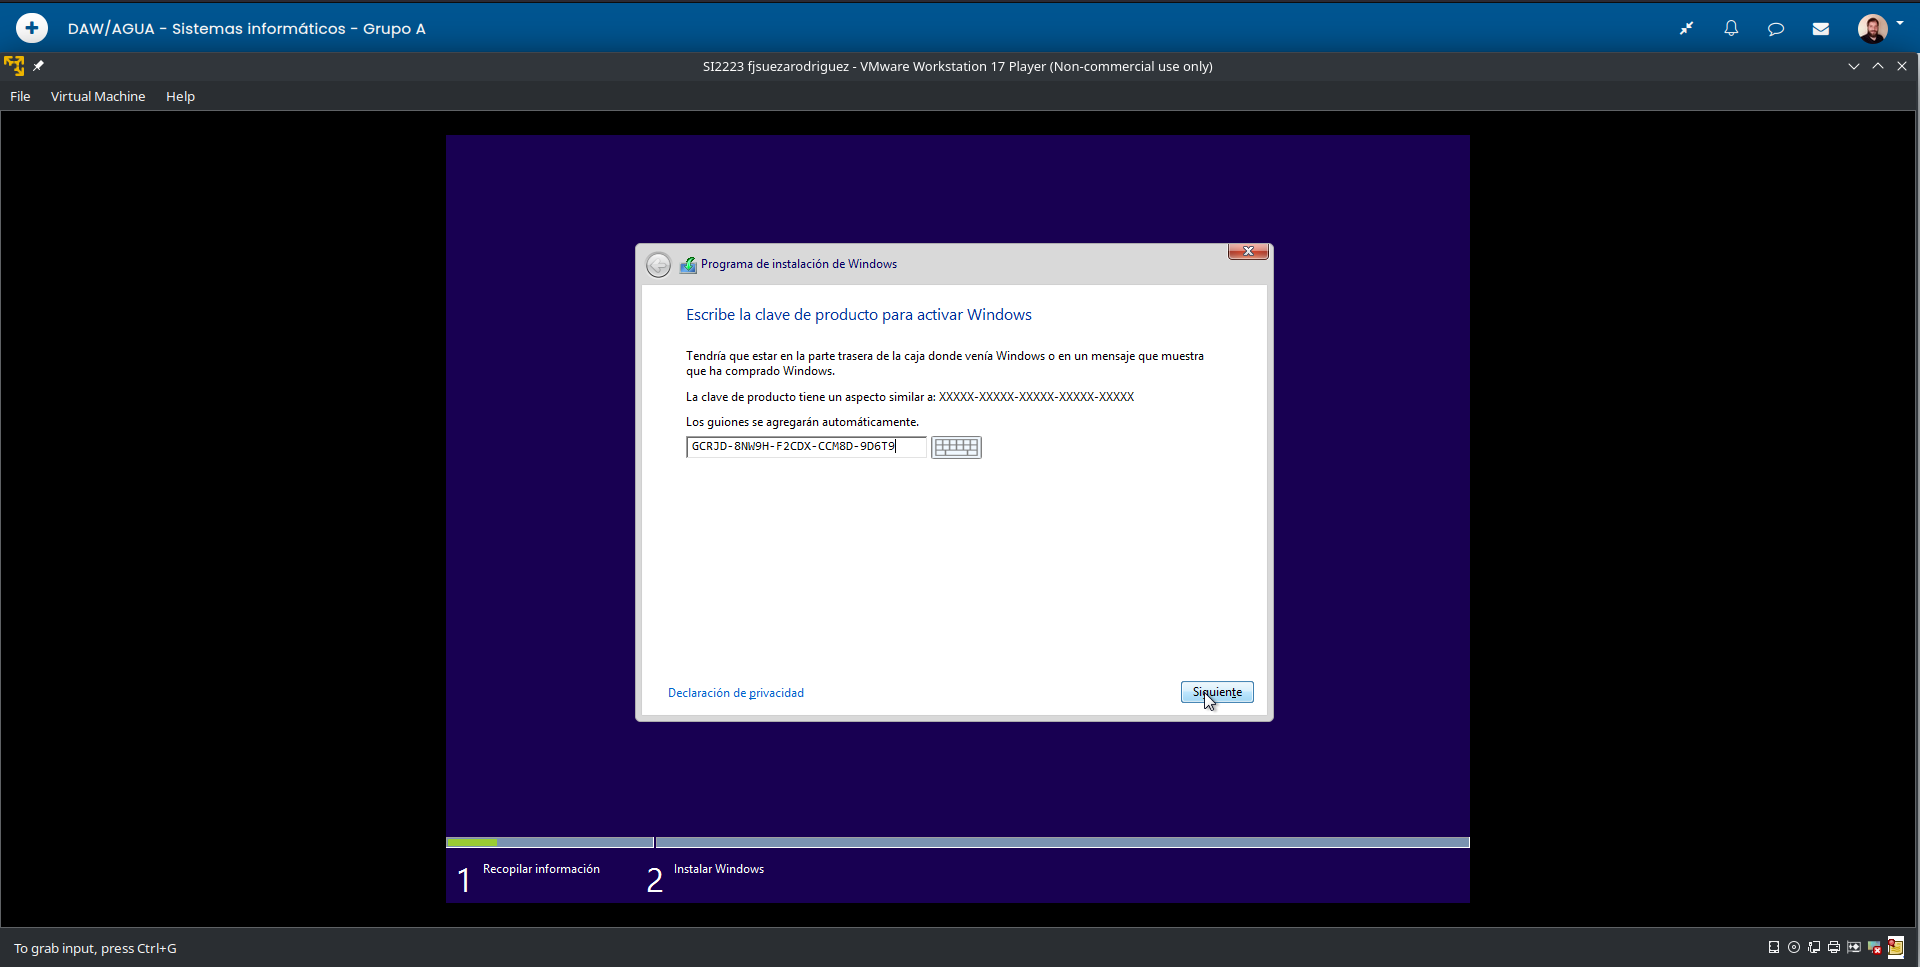
\includegraphics[scale=0.23]{windows8-install-3.png}
        \caption{Introducción del número de producto en Windows 8.1}
    \end{figure}

    \item Una vez introducida la clave del producto, se nos mostrará el gestor de particiones de la instalación. Aquí, podremos elegir realizar la instalación en todo el disco duro o crear particiones de éste y realizar la instalación en dichas particiones.

    En nuestro caso, vamos a crear una partición de 25 GB para la instalación de Windows 8.1. Además de esta partición, el sistema creará otras con propósitos específicos. En la siguiente captura vemos como ha quedado la tabla de particiones después de crear nuestra partición.

    \begin{figure}[H]
        \centering
        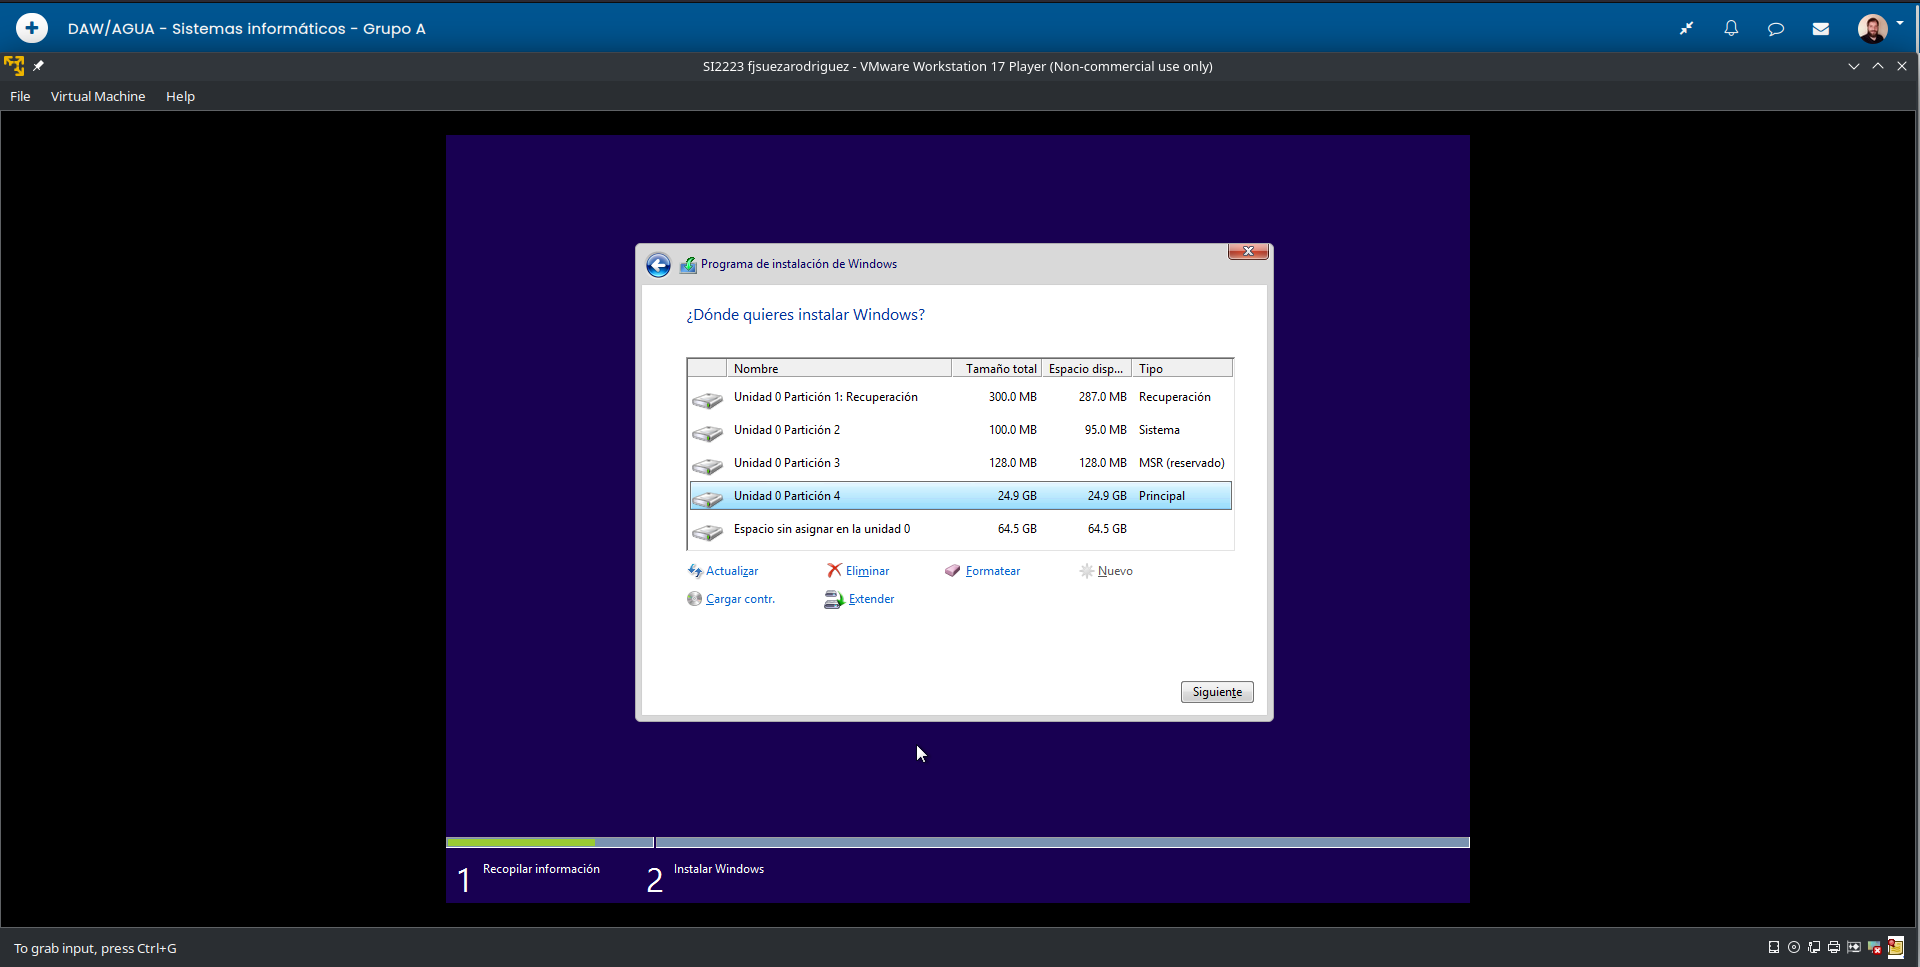
\includegraphics[scale=0.23]{windows8-install-4.png}
        \caption{Particionado del disco duro en la instalación de Windows 8.1}
    \end{figure}

    Como podemos ver, no solo se ha creado nuestra partición de 25 GB, si no se que han creado otras, las cuales pasamos a describir a continuación:

    \begin{itemize}
        \item \textbf{Partición 1: Recuperación}: Partición que se usa para la recuperación del sistema, en caso de que este no pueda arrancar y que permite restablecer los valores por defecto de este.
        \item \textbf{Partición 2: Sistema}: Esta partición es donde Windows almacena los archivos relativos a la inicialización del sistema, incluyendo el boot manager y todos los archivos relativos a este.
        \item \textbf{Partición 3: MSR}: esta partición, llamada \textbf{Microsoft Reserved}, y contiene información relativa al resto de partición, para ser empleada por aplicaciones de Microsoft.
        \item \textbf{Partición 4: Primaria}: es la partición que hemos creado para alojar el sistema operativo y todos los datos que queramos almacenar en el.
    \end{itemize}

    \item A continuación, se realizará la \textbf{copia de archivos} y la instalación. Una vez finalizada, se nos mostrarán una serie de ventanas para realizar una configuración básica del sistema, como elegir el color de la interfaz y otra serie de configuraciones, las cual podemos elegir realizarlas de forma automática o personalizada. Nosotros las hemos realizado de forma automatizada.

    Tras esta configuración, podremos introducir nuestra cuenta Microsoft para que quede ligada al sistema operativo. En nuestro caso, no vamos a usar esta opción y vamos a crear una cuenta local de usuario con los datos especificados en el enunciado, es decir, con el nombre de usuario \textbf{fjsuezarodriguez} y pa contraseña \textbf{admin2223}, como podemos ver en la siguiente captura.

    \begin{figure}[H]
        \centering
        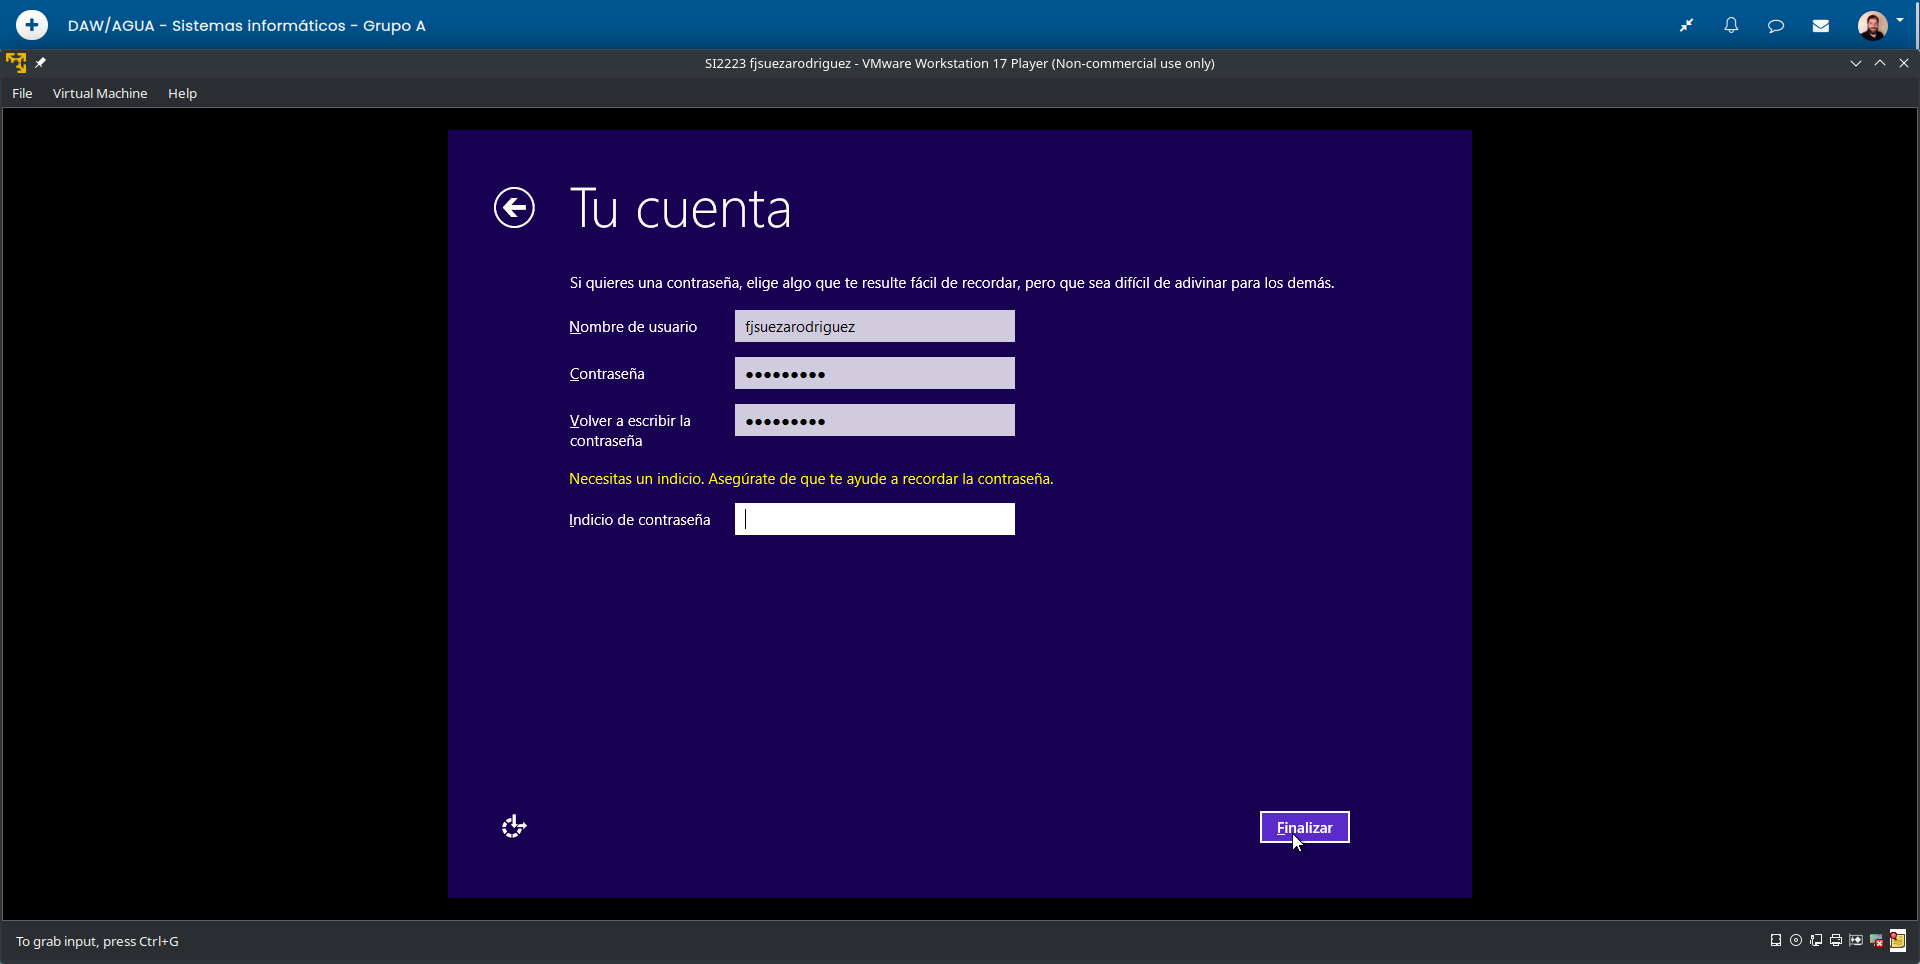
\includegraphics[scale=0.23]{windows8-install-5.png}
        \caption{Creación de usuario local durante la instalación de Windows 8.1}
    \end{figure}

    \item Tras este último paso, el sistema realizará de forma automática la instalación de algunas aplicaciones y algunas configuraciones ´y el sistema se habrá instalado correctamente.

    En la siguiente captura, se muestra Windows 8.1 funcionando correctamente en VMWare. Se muestra además la ventana con información sobre el sistema.

    \begin{figure}[H]
        \centering
        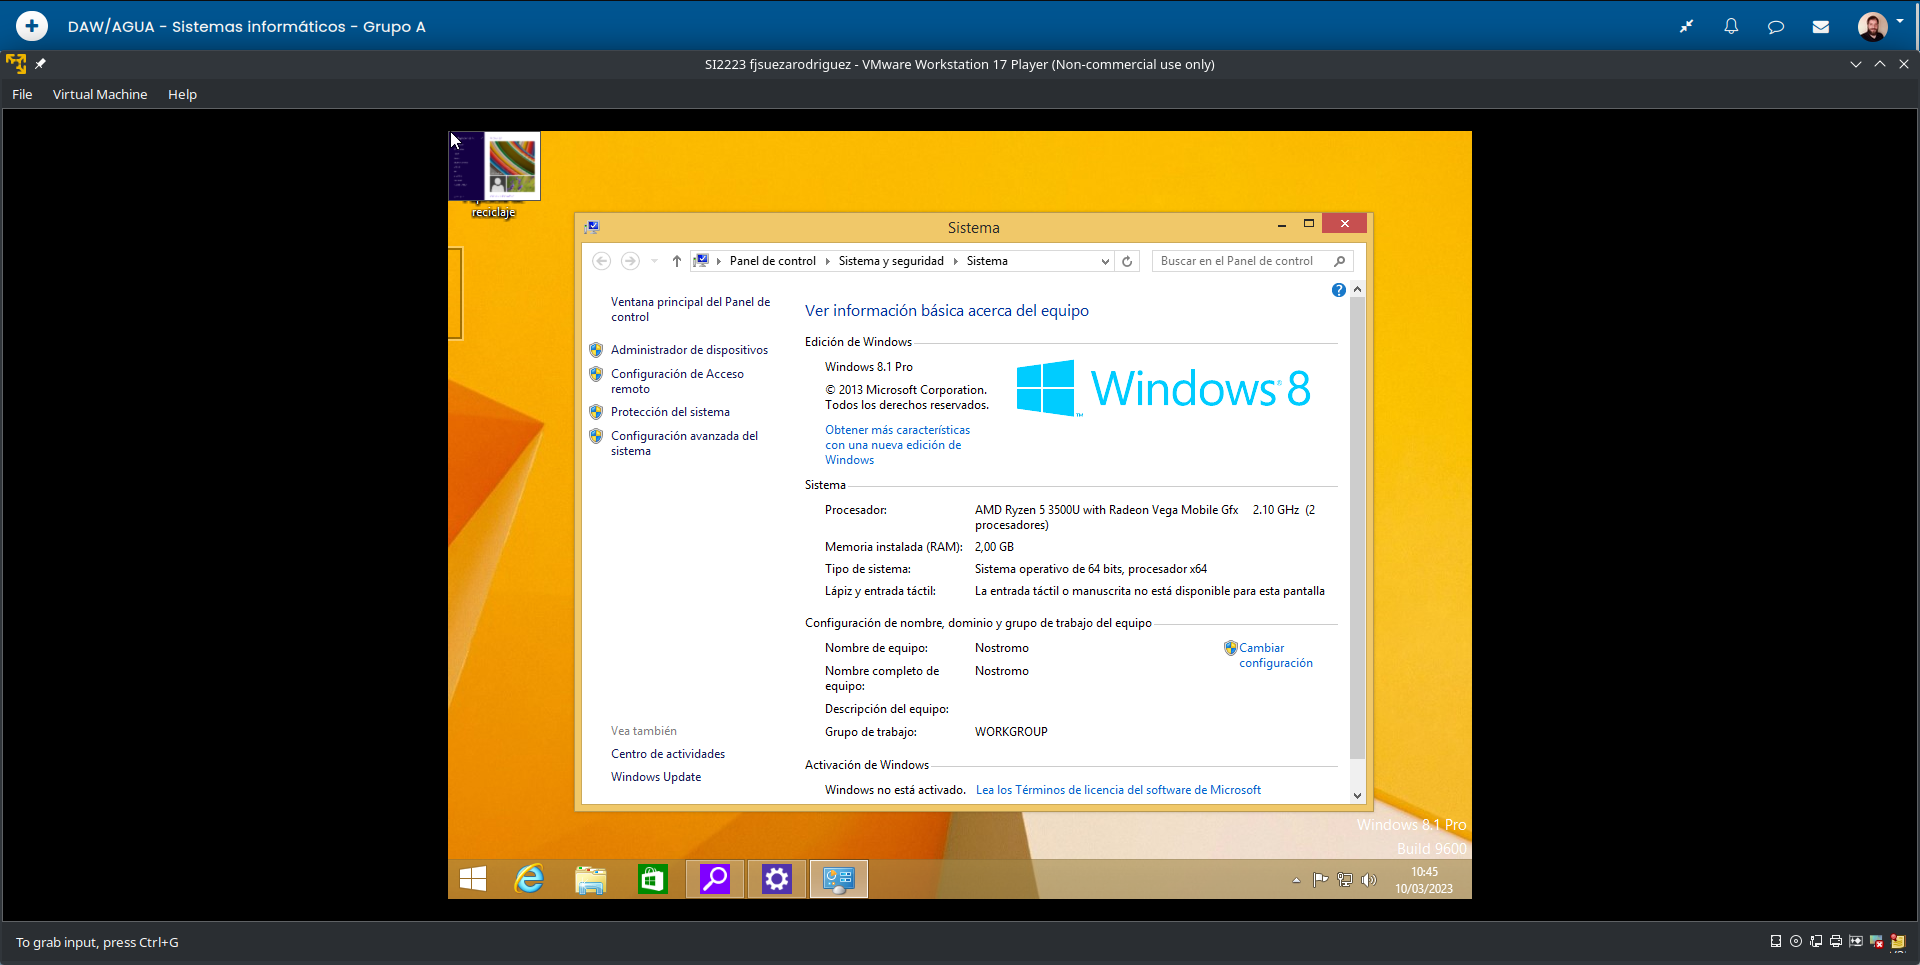
\includegraphics[scale=0.23]{windows8-install-6.png}
        \caption{Windows 8.1 instalado correctamente}
    \end{figure}
\end{enumerate}




% Bibliography

\newpage
\bibliography{citas}
\bibliographystyle{unsrt}

\end{document}